

\subsection{as\_memreader}\label{ch:07-basic-mods-in_out-memreader}

\secauthor{Alexander Zoellner}

\subsubsection{Brief Description}
The \texttt{as\_memreader} is a hardware module for efficiently transferring data from main memory to the FPGA.
The module utilizes a bus master interface to memory and an \textit{as\_stream} interface to programmable logic.
It transfers chunks of data , so called \textit{sections}, by using burst accesses whenever possible.
\textit{Sections} are defined by a start address and size.
Multiple \textit{sections} are also supported, which may include a constant offset (i.e. the difference between the start address of two consecutive \textit{sections}) in between, allowing to read rectangular sub-images or skipping certain parts of data layouts.
In order to decrease the amount of time spent idle, the following \textit{section} can be programmed during an ongoing operation by overwriting the hardware registers of the \texttt{as\_memreader} and setting its \texttt{go} flag again.
The module proceeds with the next data transfer after the current section has been completed, i.e. all data has been read.
The module provides a register for tracking the progress of the current \textit{section}, which holds the next address the module is going to read from.

\subsubsection{Architecture}

Figure~\ref{fig:memreader} shows the architecture of the \texttt{as\_memreader} module in simplified form to emphasize the main parts of the module, which are required for performing data transfers. 
The \texttt{as\_memreader} uses a \textit{Master Interface} for obtaining data from memory. 
This interface comprises only signals which are required for configuring the access to memory, such as the number of bytes to be transferred or when to start a data transfer. 
The actual memory bus access is performed by a \textit{Bus Translation} module, which is connected to the memory bus interface and the \texttt{as\_memreader}. 
Data is intermediately stored in a \textit{FIFO Buffer} first, before passing it to the subsequent hardware module. 
As aforementioned, the memory modules usually transfer a chunk of data at once, utilizing burst accesses. 
However, the subsequent hardware module may not be able to handle the amount of data at the same pace as the memory module. 
The \textit{FIFO Buffer} is used to match the processing speed of the subsequent module, by being able to temporarily suspending data transfers towards the module. 
The \texttt{as\_memreader} continuous to request data from memory, as long as the fill level of the \textit{FIFO Buffer} has not reached a certain threshold. 
Hardware modules are connected to the \texttt{as\_stream} (see Chapter~\ref{ch:05-03-interfaces-as_stream}) interface of the \texttt{as\_memreader}. 
For configuring the \texttt{as\_memreader}, a \textit{Register Interface} is utilized, which provides a number of hardware registers. 
These registers can be accessed by hardware and software alike, for exchanging control and status information. 
During an ongoing operation, certain information must not be changed for the \texttt{as\_memreader} module to operate correctly. 
For this reason, information regarding the specifics of the operation, such as number of \textit{sections} or its size, have to be kept stable. 
This is accomplished by copying critical information to \textit{Shadow Registers} at the start of an operation. 
As a side effect, this allows the software to replace the associated hardware registers during an ongoing operation, which is used for queuing the subsequent operation for transferring data. 
The \textit{Memory State Machine} controls the data flow and operation within the \texttt{as\_memreader} module. 
This part is responsible for determining the point at which the contents of the \textit{Shadow Registers} are replaced, publishing
status information to software via the Register Interface as well as accepting control information from it. 
For the actual data transfer, the \textit{Memory State Machine} is responsible for setting the appropriate signals at its \textit{Master Interface} and \texttt{as\_stream} interface, depending on the fill level of the \textit{FIFO Buffer}. 
Additionally, it evaluates the \texttt{as\_stream} signal for the \texttt{as\_memreader}. 
The \textit{Address Generator}, as the name suggests, calculates the address required for the individual memory accesses as well as the number of bytes to be transferred. 
The required information are obtained from the \textit{Shadow Registers}. 
Towards software, the address used for the next data transfer is published to software via the \textit{Register Interface}.

\begin{figure}[ht]
    \centering
    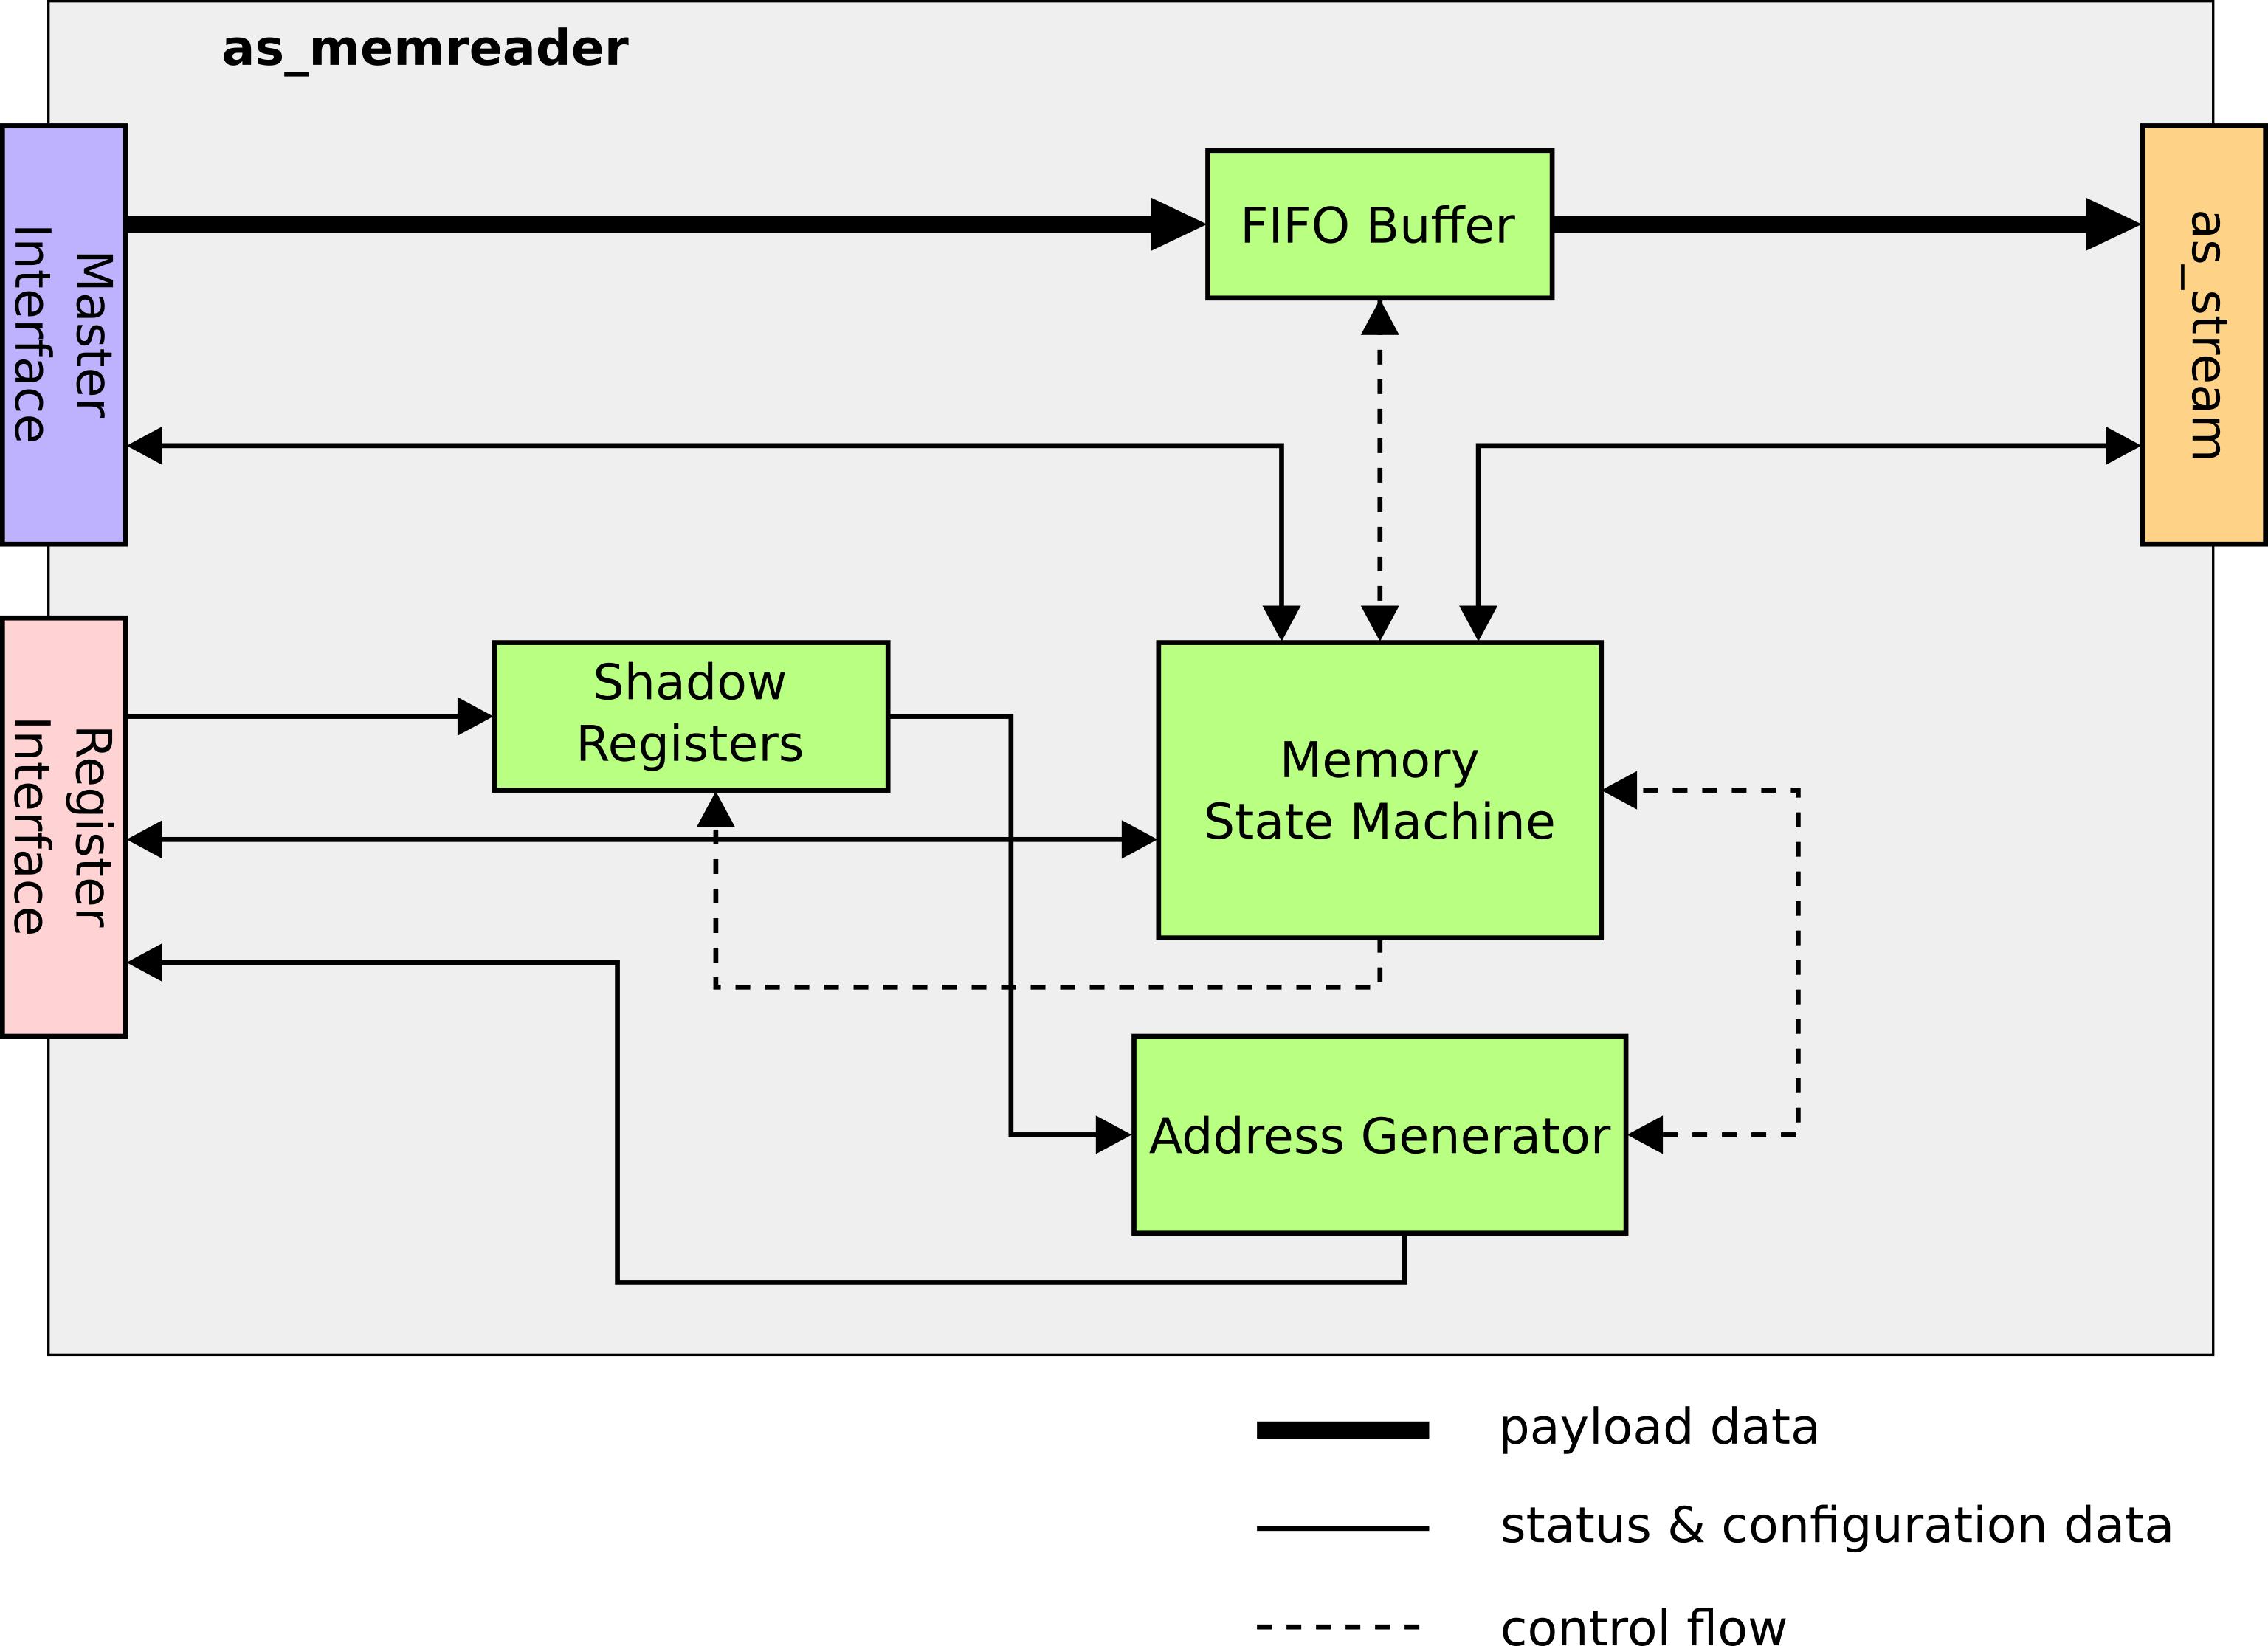
\includegraphics[width=0.8\linewidth,clip]{figs/memreader.png}
    \caption{Architecture of the \texttt{as\_memreader} module}
    \label{fig:memreader}
\end{figure}

\subsubsection{Pre-Synthesis Options}

% TBD(AZ/alle): Diesen Teil und die Layouts sollten wir in einem Meeting
%    diskutieren. @AZ: Sinnvoll ist, meine Kommentare unten vorher noch 
%    einzubauen.

\begin{longtable}[ht]{|l|l|l|}
    \hline
    \multicolumn{1}{|c|}{\textbf{Name}} & \multicolumn{1}{c|}{\textbf{Range}} & \multicolumn{1}{c|}{\textbf{Description}}\\
    \hline
    
    \small{REGISTER\_BIT\_WIDTH} & Positive integer value & \parbox{5cm}{\ \\
        Bit width for the slave registers used by this module (usually 32 bit).\vspace{0.3em}
    }\\
    \hline
    
    \small{DOUT\_WIDTH} & Positive integer value & \parbox{5cm}{\ \\
        Bit width of the data port of this module.\\
        Currently uses the same bit width as the memory bus interface (usually 32 or 64 bit).\vspace{0.3em}
    }\\
    \hline
    
    \small{MEMORY\_DATA\_WIDTH} & Positive integer value & \parbox{5cm}{\ \\
        Bit width of the data port to memory.\\
        Depends on the setting of the memory bus (usually 32 or 64 bit).\vspace{0.3em}
    }\\
    \hline
    
    \small{MEM\_ADDRESS\_BIT\_WIDTH} & Positive integer value & \parbox{5cm}{\ \\
        Bit width of the address port of the memory bus.
        Depends on the memory bus interface (usually 32 bit).\vspace{0.3em}
    }\\
    \hline
    
    \small{BURST\_LENGTH\_BIT\_WIDTH} & Positive integer value & \parbox{5cm}{\ \\
        Bit width of the memory bus to configure the burst size (currently 12 bits).\vspace{0.3em}
    }\\
    \hline
    
    \small{MAX\_PLATFORM\_BURST\_LENGTH} & Positive integer value & \parbox{5cm}{\ \\
        Highest possible burst length support by the memory bus in bytes (currently: 256).\vspace{0.3em}
    }\\
    \hline
    
    \small{FIFO\_NUMBER\_OF\_BURSTS} & Positive integer value & \parbox{5cm}{\ \\
        Minimum size of the internal data fifo. Actual size is to the power of 2 required for fitting the chosen size.\vspace{0.3em}
    }\\
    \hline
    
    \small{SUPPORT\_MULTIPLE\_SECTIONS} & Boolean & \parbox{5cm}{\ \\
        Enables regular address jumps for reading data from memory.\vspace{0.3em}
    }\\
    \hline
    
    \small{SUPPORT\_VARIABLE\_BURST\_LENGTH} & Boolean & \parbox{5cm}{\ \\
        Allows to configure actual burst length at runtime.\vspace{0.3em}
    }\\
    \hline
    
    \small{SUPPORT\_INTERRUPTS} & Boolean & \parbox{5cm}{\ \\
        Allows the module to generate interrupt events.\vspace{0.3em}
    }\\
    \hline
    
    \small{SUPPORT\_DONE\_IRQ\_SOURCE} & Boolean & \parbox{5cm}{\ \\
        Module generates an interrupt event at the end of a \textit{section}.\\
        \small{SUPPORT\_INTERRUPTS} has to be enabled.\vspace{0.3em}
    }\\
    \hline
    
\end{longtable}

\subsubsection{Register Space}

\begin{longtable}[ht]{|l|l|l|l|}
    \hline
    \multicolumn{1}{|c|}{\textbf{Name}} & \multicolumn{1}{c|}{\textbf{Relative Address}} & \multicolumn{1}{c|}{\textbf{Width}} & \multicolumn{1}{c|}{\textbf{Description}}\\
    \hline
    
    \texttt{state/control} & 0x0 & 32 & \parbox{7cm}{\ \\
        Status information of the \texttt{as\_memreader} and controlling the operation of the module. The lower half of the register is used for status information, the upper half for configuration.\vspace{0.3em}
    }\\
    \hline
    
    \texttt{section addr} & 0x4 & 32 & \parbox{7cm}{\ \\
        Memory address at which the module starts to read data from.\vspace{0.3em}
    }\\
    \hline
    
    \texttt{section offset} & 0x8 & 32 & \parbox{7cm}{\ \\
        Address offset in byte for regular address jumps. The offset is the distance between the start addresses of two consecutive \textit{sections}.\vspace{0.3em}
    }\\
    \hline
    
    \texttt{section size} & 0xC & 32 & \parbox{7cm}{\ \\
        Size of a \textit{section} in byte to be read from memory. The size has to be a multiple of the configured data bus width in byte.\vspace{0.3em}
    }\\
    \hline
    
    \texttt{section count} & 0x10 & 32 & \parbox{7cm}{\ \\
        Number of \textit{sections}. If \texttt{SUPPORT\_MULTIPLE\_SECTIONS} is not set, this register is ignored and a single \textit{section} is assumed.\\
        Otherwise, an address jump is performed between two consecutive \textit{sections}.\vspace{0.3em}
    }\\
    \hline
    
    \texttt{max burst length} & 0x14 & 32 & \parbox{7cm}{\ \\
        Number of bytes to be requested for a single memory bus access.\\
        Has to be a multiple of \texttt{MEMORY\_DATA\_WIDTH} and must not exceed \texttt{MAX\_PLATFORM\_BURST\_LENGTH}.\vspace{0.3em}
    }\\
    \hline
    
    \texttt{current hw addr} & 0x18 & 32 & \parbox{7cm}{\ \\
        Next memory address the module is going to read from.\\
        If the \texttt{as\_memreader} is not programmed this address is 0x0.\\
        For multiple \textit{sections}, it points to the last \textit{section} start address + offset after the last \textit{section} has been served.\vspace{0.3em}
    }\\
    \hline
    \caption{Register overview of the \texttt{as\_memreader} module.}
\end{longtable}


\begin{longtable}[ht]{|l|l|l|l|l|}
    \hline
    \multicolumn{1}{|c|}{\textbf{Field Name}} & \multicolumn{1}{c|}{\textbf{Bit Index}} & \multicolumn{1}{c|}{\textbf{Type}} & \multicolumn{1}{c|}{\textbf{Reset Value}} & \multicolumn{1}{c|}{\textbf{Description}}\\
    \hline
    
    \texttt{go} & 17 & wo & 0x0 & \parbox{5cm}{\ \\
        If set, the \texttt{as\_memreader} starts transferring data to memory.\vspace{0.3em}
    }\\
    \hline
    
    \texttt{reset} & 16 & wo & 0x0 & \parbox{5cm}{\ \\
        Resets the module and clears all remaining data in the \textit{FIFO Buffer}.\vspace{0.3em}
    }\\
    \hline
    
    \texttt{pending go} & 5 & ro & 0x0 & \parbox{5cm}{\ \\
        If set, the next data transfer has already been programmed.\vspace{0.3em}
    }\\
    \hline
    
    \texttt{busy} & 1 & ro & 0x0 & \parbox{5cm}{\ \\
        The \texttt{as\_memreader} is currently operating.\vspace{0.3em}
    }\\
    \hline
    
    \texttt{ready} & 0 & ro & 0x0 & \parbox{5cm}{\ \\
        The \texttt{as\_memreader} is currently idle.\vspace{0.3em}
    }\\
    \hline
    \caption{Bit field overview of the combined \texttt{state/control} register of the \texttt{as\_memreader}.}
    \label{table:memreader-state-fields}
\end{longtable}


\begin{longtable}[ht]{|l|l|l|l|l|}
    \hline
    \multicolumn{1}{|c|}{\textbf{Field Name}} & \multicolumn{1}{c|}{\textbf{Bit Index}} & \multicolumn{1}{c|}{\textbf{Type}} & \multicolumn{1}{c|}{\textbf{Reset Value}} & \multicolumn{1}{c|}{\textbf{Description}}\\
    \hline
    
    \texttt{section address} & 31:0 & wo & 0x0 & \parbox{5cm}{\ \\
        Start address for reading data from memory.\vspace{0.3em}
    }\\
    \hline
    
    \caption{Bit field overview of the \texttt{section addr} register of the \texttt{as\_memreader}.}
    \label{table:memreader-section_addr-fields}
\end{longtable}


\begin{longtable}[ht]{|l|l|l|l|l|}
    \hline
    \multicolumn{1}{|c|}{\textbf{Field Name}} & \multicolumn{1}{c|}{\textbf{Bit Index}} & \multicolumn{1}{c|}{\textbf{Type}} & \multicolumn{1}{c|}{\textbf{Reset Value}} & \multicolumn{1}{c|}{\textbf{Description}}\\
    \hline
    
    \texttt{section offet} & 31:0 & wo & 0x0 & \parbox{5cm}{\ \\
        The offset is the distance between two start addresses in byte.\vspace{0.3em}
    }\\
    \hline
    
    \caption{Bit field overview of the \texttt{section offset} register of the \texttt{as\_memreader}.}
    \label{table:memreader-section_offset-fields}
\end{longtable}


\begin{longtable}[ht]{|l|l|l|l|l|}
    \hline
    \multicolumn{1}{|c|}{\textbf{Field Name}} & \multicolumn{1}{c|}{\textbf{Bit Index}} & \multicolumn{1}{c|}{\textbf{Type}} & \multicolumn{1}{c|}{\textbf{Reset Value}} & \multicolumn{1}{c|}{\textbf{Description}}\\
    \hline
    
    \texttt{section size} & 31:0 & wo & 0x0 & \parbox{5cm}{\ \\
        Size of a \textit{section} in byte to be read from memory.\vspace{0.3em}
    }\\
    \hline
    
    \caption{Bit field overview of the \texttt{section size} register of the \texttt{as\_memreader}.}
    \label{table:memreader-section_size-fields}
\end{longtable}


\begin{longtable}[ht]{|l|l|l|l|l|}
    \hline
    \multicolumn{1}{|c|}{\textbf{Field Name}} & \multicolumn{1}{c|}{\textbf{Bit Index}} & \multicolumn{1}{c|}{\textbf{Type}} & \multicolumn{1}{c|}{\textbf{Reset Value}} & \multicolumn{1}{c|}{\textbf{Description}}\\
    \hline
    
    \texttt{section count} & 31:0 & wo & 0x0 & \parbox{5cm}{\ \\
        Number of \textit{sections}.\vspace{0.3em}
    }\\
    \hline
    
    \caption{Bit field overview of the \texttt{section count} register of the \texttt{as\_memreader}.}
    \label{table:memreader-section_count-fields}
\end{longtable}


\begin{longtable}[ht]{|l|l|l|l|l|}
    \hline
    \multicolumn{1}{|c|}{\textbf{Field Name}} & \multicolumn{1}{c|}{\textbf{Bit Index}} & \multicolumn{1}{c|}{\textbf{Type}} & \multicolumn{1}{c|}{\textbf{Reset Value}} & \multicolumn{1}{c|}{\textbf{Description}}\\
    \hline
    
    \texttt{max burst length} & 31:0 & wo & 0x0 & \parbox{5cm}{\ \\
        Number of bytes to be requested for a single memory bus access.\vspace{0.3em}
    }\\
    \hline
    
    \caption{Bit field overview of the \texttt{max burst length} register of the \texttt{as\_memreader}.}
    \label{table:memreader-burst-fields}
\end{longtable}


\begin{longtable}[ht]{|l|l|l|l|l|}
    \hline
    \multicolumn{1}{|c|}{\textbf{Field Name}} & \multicolumn{1}{c|}{\textbf{Bit Index}} & \multicolumn{1}{c|}{\textbf{Type}} & \multicolumn{1}{c|}{\textbf{Reset Value}} & \multicolumn{1}{c|}{\textbf{Description}}\\
    \hline
    
    \texttt{current hw addr} & 31:0 & ro & 0x0 & \parbox{5cm}{\ \\
        Next address the \texttt{as\_memreader} is going to read from.\vspace{0.3em}
    }\\
    \hline
    
    \caption{Bit field overview of the \texttt{current hw addr} register of the \texttt{as\_memreader}.}
    \label{table:memreader-cur_hw-fields}
\end{longtable}

\subsubsection{Behavior}
The bit fields of the \texttt{control} and \texttt{state} registers are also represented internally within the module by signals with the same name.
When referring to the bit field, the name is written in lower case and in upper case for the signal.
Flags refer to the bit fields.

% Start up and reset (during reset, post reset)
When the module receives a reset request, either by using the hardware port or the \texttt{reset} flag of the \textit{State Control} register, ongoing bus accesses are terminated and all internally stored configuration settings are cleared after a single clock cycle.
Additionally, the module requests to clear the \texttt{go} and \texttt{reset} field.
The configuration registers towards software are left as is.
Simultaneously, the data in the \textit{FIFO Buffer} is discarded and the address generator is reset.
The reset persists only for one clock cycle if it has been requested by software, otherwise up to the point it is lifted by hardware.
During the reset, neither of the modules' status flags is set.
After the reset has been lifted, the \texttt{as\_memreader} assumes its idle state.


% Operation
In the modules' idle state, the \texttt{ready} flag is set and the configuration registers are continuously copied into internal shadow registers.
Upon setting the \texttt{go} field, the current configuration is used for setting up data transfers after one clock cycle.
Further, the \texttt{ready} flag is unset and the \texttt{busy} flag is set instead, which is kept throughout the whole operation.
The \texttt{as\_memreader} requests the slave logic to clear the \texttt{go} flag and starts accessing the master memory bus interface.
During operation, the configuration registers can be overwritten and \texttt{go} flag set again, to seamlessly queue the next data transfer.
If the \texttt{go} flag was set in this manner, the module sets its \texttt{PENDING GO} signal.
Since the \texttt{as\_memreader} copies the configuration only at the start, it would be possible to change the configuration for the following transfer after having already set the \texttt{go} flag again.
However, it is strongly recommended to configure the data transfer before queuing the next transmission.
As soon as the \texttt{as\_memreader} has read all requested data for the current operation, it sets the \texttt{ready} flag again and returns to its idle state.
Here, the \texttt{busy} and \texttt{ready} flag are set simultaneously for a single clock cycle, which is exclusively used if another hardware module interfaces the \texttt{as\_memwriter} instead of software.
This is mainly for backwards compatibility and may be subject to change in the future.
If the next \texttt{GO} has already been set when entering the idle state, the module proceeds in the aforementioned manner without delay.
The \texttt{PENDING GO} (since \texttt{GO} is unset) is unset again.


% Stall
The \texttt{as\_memreader} is a \textit{stall-absorbing} module (see Chapter~\ref{05-03-stall}), which means it accepts requests to suspend data transfers by the following module.
After receiving a stall request, the \texttt{as\_memreader} stops transferring data at its \textit{as\_stream} output interface on the following clock cycle, until the stall is lifted again.
Since the module utilizes a \textit{FIFO Buffer}, it continues to read data from memory if there is remaining space.
The fifo is considered full, if it can only hold the equivalent of one additional maximal possible burst length amount of data.
Since the actually utilized burst length may vary (if \texttt{SUPPORT\_VARIABLE\_BURST\_LENGTH} is set), this method allows to prevent \textit{FIFO Buffer} overflow without having to check the precise amount of space left for each memory bus request.
This method has mainly been chosen to prevent the module from inefficiently reading multiple small amounts of data in order to utilize the whole \textit{FIFO Buffer}.
Instead, if the aforementioned threshold has been reached, the \texttt{as\_memreader} suspends reading data from memory until the \textit{FIFO Buffer} has output some data.
As a side effect, some FPGA area has been saved which would be required for the comparison.


% Support multiple sections
The \texttt{as\_memreader} module organizes its data transfers in one or more \textit{sections}, where each one is a physically continuous chunk of data in memory.
If more than one \textit{section} is required, the configuration option \texttt{SUPPORT\_MULTIPLE\_SECTIONS} has to be set at synthesis time.
The register \textit{Section Address} defines the memory address of the first \textit{section}, whereas \textit{Section Offset} is used for the following ones.
The latter is the difference of the start addresses of two consecutive \textit{sections}.
For example, if the first \textit{section} starts at the hexadecimal address "0x2000" and the following one at "0x5000", an offset of "0x3000" has to be configured.
The third \textit{section} would start at address "0x8000".
The number of \textit{sections} are chosen by writing a number greater 1 to the register \textit{Section Count}.
The size of a single \textit{section} is configured by using \textit{Section Size}.
When using more than one \textit{section}, the configured size should not exceed the offset, since it would result in partially overwriting the preceding \textit{section} with the following one.
If the value of \textit{Section Size} is less than \textit{Section Offset}, the difference between two \textit{sections} is skipped.
Assuming the above example with a size of "0x2200", the address range from "0x4200" to "0x4fff" is skipped and therefore not read from memory.
This method can be used for reading a sub-image from memory or skipping regular areas of a certain data layout.
If \texttt{SUPPORT\ MULTIPLE\ SECTIONS} is not set, \textit{Section Offset} and \textit{Section Count} are ignored and a single \textit{section} is assumed.


% Current hw addr
After starting the operation of the \texttt{as\_memreader} for the first time by setting the \texttt{GO} signal, the module continuously provides the current physical memory address of the \textit{Address Generator} to the software.
This address is the one used for the next memory access but might not have been processed yet.
It is stored within the hardware register \texttt{current hw addr}.
At the end of the operation of the \texttt{as\_memreader}, the address within this register points at the first address following the current \textit{section} if \texttt{SUPPORT\_MULTIPLE\_SECTIONS} has been set to "false".
Otherwise, it points at the start address of the following \textit{section}, although it is not used.
This is due to the fact, that the address is incremented by the \textit{offset} after each \textit{section}, where the last one is not handled separately.
The address is only updated during the operation of the \texttt{as\_memreader} and therefore is also not cleared once it has finished its operation.
However, performing a \textit{reset} on the module, either by hardware or software, clears the register.


% Variable burst length
The \texttt{as\_memreader} preferably utilizes burst accesses to read a chunk of memory at once, since requesting the memory bus requires a considerable overhead.
By using bursts, the number of bus accesses and therefor required overhead can be reduced.
The number of bytes used for a burst access can be configured using the register \textit{Maximal Burst Length}.
The configured number of bytes written to this register has to be a multiple of the of the memory bus interface.
Additionally, the maximal amount of data transferred in a single burst is usually limited by the architecture, to prevent other bus masters from starving, which must not be exceeded.
If the configured \textit{Section Size} is not a multiple of \textit{Maximal Burst Length}, the \texttt{as\_memreader} module falls back to less efficient single beat accesses for the remaining bytes, if \texttt{SUPPORT\_VARIABLE\_BURST\_LENGTH} has not been set.
The module requests the number of bytes equal to the one used for the memory bus interface at a time, which is usually 4 or 8 bytes.
If \texttt{SUPPORT\_VARIABLE\_BURST\_LENGTH} has been set, however, the \texttt{as\_memreader} performs a burst access for equal to the remaining number of bytes.\newline


% Error handling
The \texttt{as\_memreader} module does not perform any kind of error handling (see Chapter~\ref{ch:05-02-interfaces-module_signals}).
Since the module is designed to actively "pull" data, a \texttt{SYNC\_ERROR} due to lost data cannot occur.
Additionally, the \texttt{as\_memreader} is not able to determine whether its received data posses a valid value and therefore does not generate a \texttt{DATA\_ERROR} either.


% as\_arbiter
Instead of directly utilizing a memory bus master, the \texttt{as\_memreader} module can also be connected to an \textit{as\_arbiter} for mapping multiple \asterics memory modules to a single memory bus master.
The \texttt{as\_memreader} requests a bus access by setting the port \texttt{mem\_req} to "1" and subsequently for the same value appearing at its \texttt{mem\_req\_ack} port.
The latter port has to be bound to "1" (high), if no \textit{as\_arbiter} is used.


% Interrupt
Optionally, the \texttt{as\_memreader} generates a high level ("1") at its \texttt{interrupt\_out} port when it finishes its configured data transfer operation, i.e. all \textit{sections} have been read from memory.
Therefor, the pre-synthesis parameters \texttt{SUPPORT\_INTERRUPTS} and \texttt{SUPPORT\_DONE\_IRQ\_SOURCE} have to be set to "true".
The signal is active for a single clock cycle and can be used for generating a hardware interrupt for the processor, by using one of the available interrupt lines.


\subsubsection{Module Driver}
In order to set up data transfers from software, a module driver, namely \texttt{as\_reader\_writer}, is provided for the \texttt{as\_memreader}.
This driver is implemented in \textit{C} and comprises a header and a source file.
Within the module driver, a number of macros are defined for calculating the offset of the hardware registers and their bit indices.
These macros can be used for interfacing the hardware registers of the \texttt{as\_memreader} manually.
Alternatively, the functions of the module driver can be used. 
The provided functions enable to utilize the functionality of the module without having to look up the appropriate macros.
Internally, the \textit{\asterics Support Library} is used for performing the actual accesses to hardware.

\subsubsection{Application Notes}
For common applications using \texttt{as\_memreader} module, the default settings for most of its pre-synthesis parameters can be used.
The only exception is \texttt{DOUT\_WIDTH} and \texttt{MEMORY\_DATA\_WIDTH} which may be adjusted to 64 bit.
The following Listing~\ref{lst:memreader_setup} shows how the \texttt{as\_memreader} module is usually set up for a bare-metal application.
For using the module with an operating system, the device driver of the \asterics framework has to be used (see Chapter~\ref{ch:04-05-software-linux}).
As a first step, the registers of the module are set by using the function \texttt{as\_reader\_writer\_init()}.
It takes two arguments, the start address of the module, which is defined in \textit{as\_hardware.h}, and a pointer to the configuration structure \texttt{as\_reader\_writer\_config\_t} defined in the header file of the module driver.
By allocating a structure of this type, the corresponding data fields can be set in advance, to configure the module at once.
If a NULL pointer is provided to \texttt{as\_reader\_writer\_init()}, the default values defined in the header file are used, which covers most applications.
The function also resets the hardware module.
The \textit{section address} and \textit{section size} have to be manually configured by the user by using \texttt{as\_reader\_writer\_set\_section\_addr()} and \texttt{as\_reader\_writer\_set\_section\_size()} respectively.
A default \textit{section size} is set by \texttt{as\_reader\_writer\_init()}, however, the value is likely to differ from what is required by the user.
Lastly, \texttt{as\_reader\_writer\_set\_go()} starts the operation.
For some applications it may be required to check whether the module has completed its operation by using \texttt{as\_reader\_writer\_is\_done()}.
The given example shows an active status polling of the device, but different methods may also be used.


\begin{footnotesize}
    \lstset{style=CStyle, caption={Using the \texttt{as\_memreader} module.}}
    \begin{lstlisting}[label=lst:memreader_setup]
    /* Define a section size; here: the resolution of an image in 
       byte */ 
    #define IMAGE_RES           640*480
    
    /* Allocate a memory area */
    void *image_address = as_malloc(IMAGE_RES);
    
    
    /******* Setting up the as_memreader module *******/
    
    /* Sets default values for burst length, etc. */
    as_reader_writer_init(AS_MODULE_BASEADDR_MEMREADER_0, NULL);
    
    /* Set the start address, where the as_memreader is supposed to 
       read from */
    as_reader_writer_set_section_addr( \
        AS_MODULE_BASEADDR_MEMREADER_0, \
        (uint32_t*) image_address);
    
    /* Set the number of bytes to be read */
    as_reader_writer_set_section_size( \
        AS_MODULE_BASEADDR_MEMREADER_0, IMAGE_RES)
    
    
    /************** Data transfer **************/
    
    /* Start the as_memreader */
    as_reader_writer_set_go(AS_MODULE_BASEADDR_MEMREADER_0);
    
    /* Wait until the as_memreader has completed the section */
    while(!as_reader_writer_is_done( \
        AS_MODULE_BASEADDR_MEMREADER_0)) {
    /* Do nothing */
    }
    \end{lstlisting}
\end{footnotesize}


\subsection{as\_memwriter} \label{ch:07-basic-mods-in_out-memwriter}

\secauthor{Alexander Zoellner}

\subsubsection{Brief Description}

The \texttt{as\_memwriter} is a hardware module for efficiently transferring data from the FPGA to main memory.
The module utilizes an \textit{as\_stream} interface to programmable logic and a bus master interface to memory.
It transfers chunks of data , so called \textit{sections}, by using burst accesses whenever possible.
\textit{Sections} are defined by a start address and size.
Multiple \textit{sections} are also supported, which may include a constant offset (i.e. the difference between the start address of two consecutive \textit{sections}) in between, allowing to write rectangular sub-images or complying to a certain data layout.
In order to decrease the amount of time spent idle, the following \textit{section} can be programmed during an ongoing operation by overwriting the hardware registers of the \texttt{as\_memwriter} and setting its \texttt{go} flag again.
The module proceeds with the next data transfer after the current \textit{section} has been completed, i.e. all data has been written.
The module provides a register for tracking the progress of the current \textit{section}, which holds the next address the module is going to read from.
Additionally, the \texttt{as\_memwriter} supports organizing data in \textit{data units}, which is a logically grouped number of bytes.
A counter, readable by software, is used for tracking the number of \textit{data units}, which have been transferred to memory.
This can be used for counting frames, image lines or any arbitrary data sets.

\subsubsection{Architecture}

Figure~\ref{fig:memwriter} shows the architecture of the \texttt{as\_memwriter} module in simplified form to emphasize the main parts of the module, which are required for performing data transfers. 
The \texttt{as\_memwriter} obtains its data via a hardware module, using the \texttt{as\_stream} interface (see Chapter~\ref{ch:05-03-interfaces-as_stream}).
The incoming data is intermediately stored in a \textit{FIFO Buffer}, in order to aggregate a certain number of bytes for performing more efficient data transfers towards memory, using \textit{bursts}.
Further, data loss is prevented in this manner, if access to the memory bus cannot be obtained right away.
If the \textit{FIFO Buffer} reaches its limit, the \texttt{as\_memwriter} requests the preceding module to suspend any further data transfers to its \texttt{as\_stream} interface.
The \texttt{as\_memwriter} utilizes a \textit{Master Interface} for transferring data to memory.
This interface comprises only signals which are required for configuring the access to memory, such as the number of bytes to be transferred or when to start a data transfer. 
The actual memory bus access is performed by a \textit{Bus Translation} module, which is connected to the memory bus interface and the \texttt{as\_memwriter}.
Occasionally, the user may not require the data of the image processing chain, which results in the \texttt{as\_memwriter} to not transfer any data to memory.
In this case, the \textit{Enable Logic} is used to discard any following data at the \texttt{as\_stream} interface, to prevent the \textit{FIFO Buffer} from overflowing.
Thus, the \texttt{as\_memwriter} does not have to request the preceding module to suspend its data transfers, since other parts of the processing chain may depend on the data (e.g. the \texttt{as\_memwriter} is only used to store intermediate results for control purposes).
For regular operation, the \textit{Enable Logic} merely forwards the data to the \textit{FIFO Buffer}.

For configuring the \texttt{as\_memwriter}, a \textit{Register Interface} is utilized, which are associated with a number of hardware registers. 
These registers can be accessed by hardware and software alike, for exchanging control and status information. 
The control information are provided by software via the \textit{Register Interface} to affect the behavior of the \texttt{as\_memwriter}.
For this reason, the appropriate hardware registers are connected to the \textit{Enable Logic} to choose whether the \texttt{as\_memwriter} is expected to discard data at its \texttt{as\_stream} interface.
The \textit{Memory State Machine} is the central part of the module and is responsible for setting up data transfers, according to the settings of the software within the hardware registers.
It also affects the \textit{Enable Logic} under certain conditions.

During an ongoing operation, certain information must not be changed, in order for the \texttt{as\_memwriter} module to operate correctly. 
For this reason, information regarding the specifics of the operation, such as number of \textit{sections} or its size, have to be kept stable. 
This is accomplished by copying critical information to \textit{Shadow Registers} at the start of an operation, which is determined by the \textit{Memory State Machine}. 
As a side effect, this allows the software to replace the associated hardware registers during an ongoing operation, which is used for queuing the subsequent operation for transferring data. 
The \textit{Address Generator} calculates the address required for the individual memory accesses as well as the number of bytes to be transferred. 
The required information are obtained from the \textit{Shadow Registers}. 
Towards software, the address used for the next data transfer is published to software via the \textit{Register Interface}.

Optionally, the \textit{Data Unit Complete Logic} can be added to the \texttt{as\_memwriter} if \texttt{SUPPORT\_DATA\_UNIT\_COMPLETE} has been set.
It is used for tracking the number of \textit{data units} which have been transferred to memory.
This number as well as the end address of the last \textit{data unit} is published to software using the \textit{Register Interface}.
For certain configurations, the \textit{Data Unit Complete Logic} also affects the \textit{Enable Logic}.


\begin{figure}[ht]
    \centering
    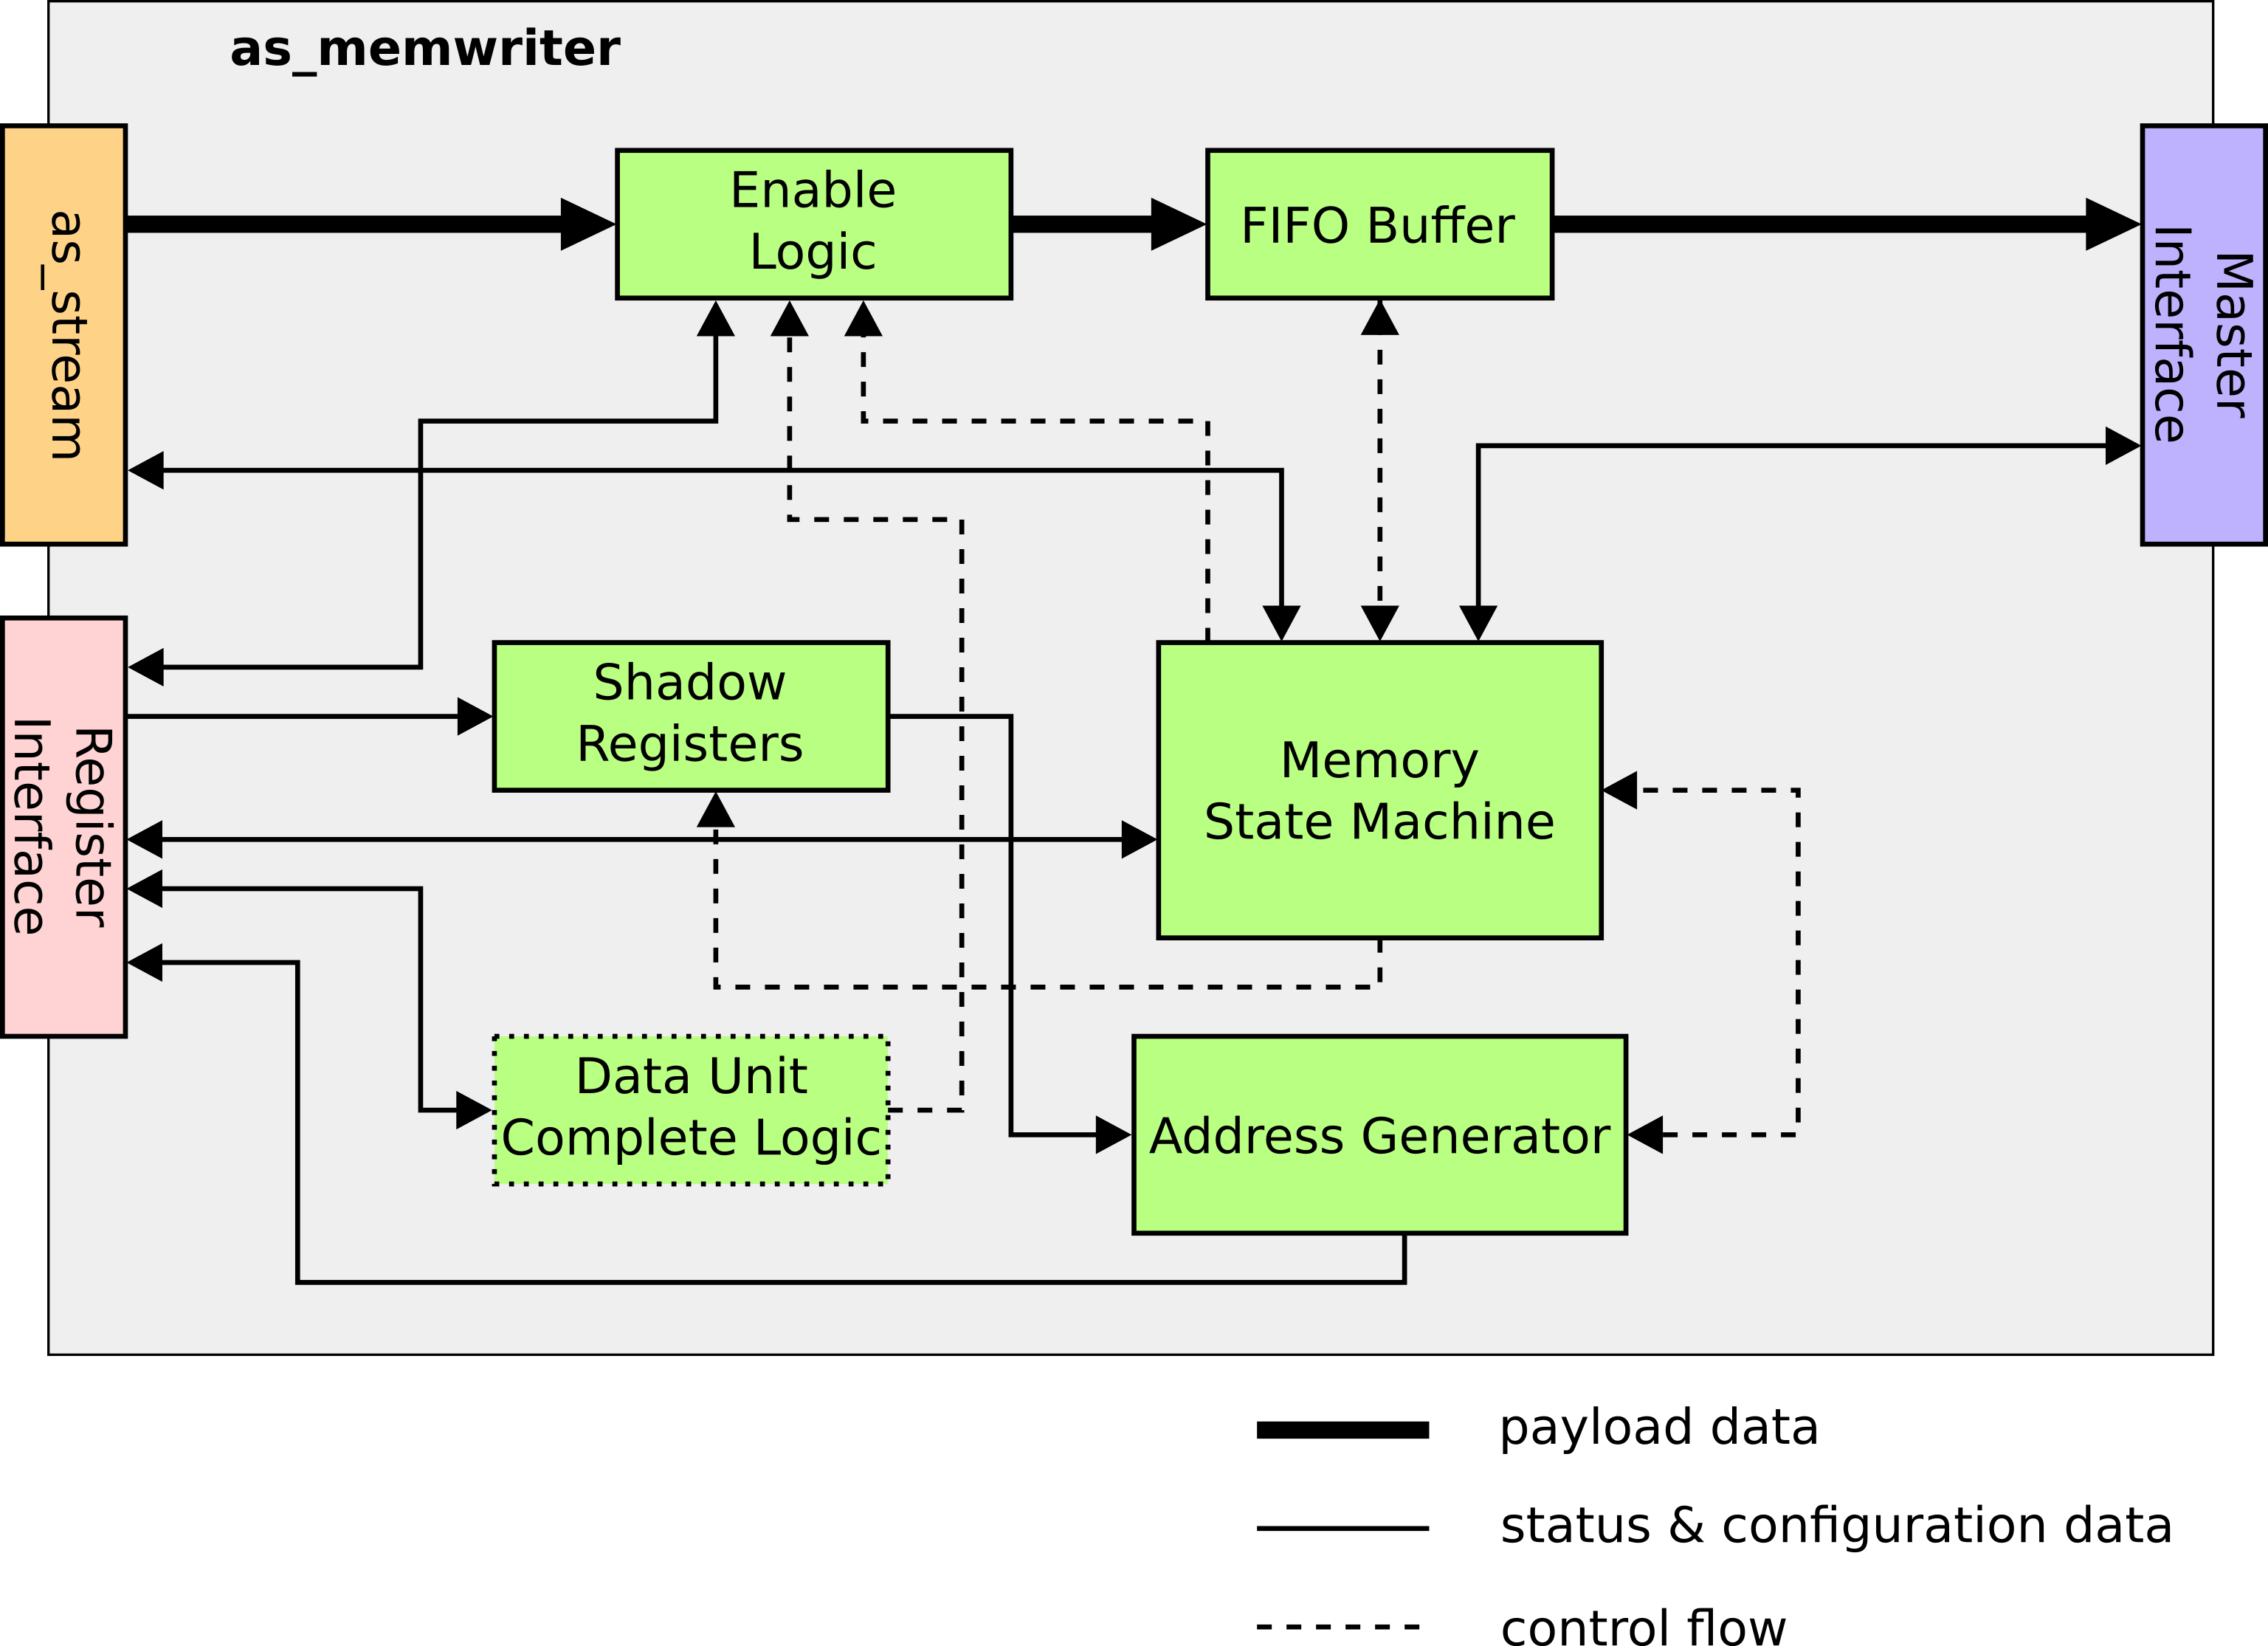
\includegraphics[width=0.8\linewidth,clip]{figs/memwriter.png}
    \caption{Architecture of the \texttt{as\_memwriter} module}
    \label{fig:memwriter}
\end{figure}

\subsubsection{Pre-Synthesis Options}

\begin{longtable}[ht]{|l|l|l|}
    \hline
    \multicolumn{1}{|c|}{\textbf{Name}} & \multicolumn{1}{c|}{\textbf{Range}} & \multicolumn{1}{c|}{\textbf{Description}}\\
    \hline
    
    \small{REGISTER\_BIT\_WIDTH} & Positive integer value & \parbox{5cm}{\ \\
        Bit width for the slave registers used by this module (usually 32 bit).\\
    }\\
    \hline
    
    \small{DOUT\_WIDTH} & Positive integer value & \parbox{5cm}{\ \\
        Bit width of the data port of this module.\\
        Currently uses the same bit width as the memory bus interface (usually 32 or 64 bit).\\
    }\\
    \hline
    
    \small{MEMORY\_DATA\_WIDTH} & Positive integer value & \parbox{5cm}{\ \\
        Bit width of the data port to memory.\\
        Depends on the setting of the memory bus (usually 32 or 64 bit).\\
    }\\
    \hline
    
    \small{MEM\_ADDRESS\_BIT\_WIDTH} & Positive integer value & \parbox{5cm}{\ \\
        Bit width of the address port of the memory bus.\\
        Depends on the memory bus interface (usually 32 bit).
    }\\
    \hline
    
    \small{BURST\_LENGTH\_BIT\_WIDTH} & Positive integer value & \parbox{5cm}{\ \\
        Bit width of the memory bus to configure the burst size (currently 12 bits).\\
    }\\
    \hline
    
    \small{MAX\_PLATFORM\_BURST\_LENGTH} & Positive integer value & \parbox{5cm}{\ \\
        Highest possible burst length support by the memory bus in bytes (currently: 256).\\
    }\\
    \hline
    
    \small{FIFO\_NUMBER\_OF\_BURSTS} & Positive integer value & \parbox{5cm}{\ \\
        Minimum size of the internal data fifo. The actual size is to the power of 2 required for fitting the chosen size.\\
    }\\
    \hline
    
    \small{SUPPORT\_MULTIPLE\_SECTIONS} & Boolean & \parbox{5cm}{\ \\
        Enables regular address jumps for reading data from memory.\\
    }\\
    \hline
    
    
    \small{SUPPORT\_INTERRUPTS} & Boolean & \parbox{5cm}{\ \\
        Allows the module to generate interrupt events.\\
    }\\
    \hline
    
    \small{SUPPORT\_DONE\_IRQ\_SOURCE} & Boolean & \parbox{5cm}{\ \\
        Module generates an interrupt event at the end of a \textit{section}.\\
        \small{SUPPORT\_INTERRUPTS} has to be enabled.\\
    }\\
    \hline
    
    \small{SUPPORT\_DUC\_IRQ\_SOURCE} & Boolean & \parbox{5cm}{\ \\
        Module generates an interrupt event at the end of a data unit.\\
        \small{SUPPORT\_INTERRUPTS} has to be enabled.\\
        \small{SUPPORT\_DATA\_UNIT\_}\\
        \small{COMPLETE} has to be enabled.\\
    }\\
    \hline
    
    \small{SUPPORT\_DATA\_UNIT\_COMPLETE} & Boolean & \parbox{5cm}{\ \\
        Module generates an interrupt event at the end of a data unit.\\
        \small{SUPPORT\_INTERRUPTS} has to be enabled.\\
    }\\
    \hline
    
    \small{UNIT\_COUNTER\_WIDTH} & Positive integer value & \parbox{5cm}{\ \\
        Bit width of the register for storing the number of data units.\\
    }\\
    \hline
    
\end{longtable}

\subsubsection{Register Space}

\begin{longtable}[ht]{|l|l|l|l|}
    \hline
    \multicolumn{1}{|c|}{\textbf{Name}} & \multicolumn{1}{c|}{\textbf{Relative Address}} & \multicolumn{1}{c|}{\textbf{Width}} & \multicolumn{1}{c|}{\textbf{Description}}\\
    \hline
    
    \texttt{state/control} & 0x0 & 32 & \parbox{7cm}{\ \\
        Status information of the \texttt{as\_memwriter} and controlling the operation of the module. The lower half of the register is used for status information, the upper half for configuration.\\
    }\\
    \hline
    
    \texttt{ section addr} & 0x4 & 32 & \parbox{7cm}{\ \\
        Memory address at which the module starts to read data from.\\
    }\\
    \hline
    
    \texttt{section offset} & 0x8 & 32 & \parbox{7cm}{\ \\
        Address offset in byte for regular address jumps. The offset is the distance between the start addresses of two consecutive \textit{sections}.\\
    }\\
    \hline
    
    \texttt{section size} & 0xC & 32 & \parbox{7cm}{\ \\
        Size of a \textit{section} in byte to be read from memory. The size has to be a multiple of the configured data bus width in byte.\\
    }\\
    \hline
    
    \texttt{section count} & 0x10 & 32 & \parbox{7cm}{\ \\
        Number of \textit{sections}. If \texttt{SUPPORT\_MULTIPLE\_SECTIONS} is not set, this register is ignored and a single \textit{section} is assumed.\\
        Otherwise, an address jump is performed between two consecutive \textit{sections}.\\
    }\\
    \hline
    
    \texttt{max burst length} & 0x14 & 32 & \parbox{7cm}{\ \\
        Number of bytes to be requested for a single memory bus access.\\
        It has to be a multiple of \texttt{MEMORY\_DATA\_WIDTH} and must not exceed \texttt{MAX\_PLATFORM\_BURST\_LENGTH}.\\
    }\\
    \hline
    
    \texttt{current hw addr} & 0x18 & 32 & \parbox{7cm}{\ \\
        Contains the next memory address the module is going to read from.\\
        If the \texttt{as\_memwriter} is not programmed this address is 0x0.\\
        For multiple \textit{sections}, it points to the last \textit{section} start address + offset after the last \textit{section} has been served.\\
    }\\
    \hline
    
    \parbox{3cm}{\texttt{last data unit complete addr}} & 0x1C & 32 & \parbox{7cm}{\ \\
        Following address after a data unit has been written to memory.\\
        \texttt{SUPPORT\_DATA\_UNIT\_}\small{COMPLETE} has to be set. Otherwise the value of this register is always 0x0.\\
    }\\
    \hline
    
    \texttt{current unit count} & 0x20 & 32 & \parbox{7cm}{\ \\
        Number of transferred data units to memory.\\
        \texttt{SUPPORT\_DATA\_UNIT\_}\small{COMPLETE} has to be set. Otherwise the value of this register is always 0x0.\\
        The actual number of utilized bits of this register depend on the setting of \texttt{UNIT\_COUNTER\_WITDH}, up to 32.
    }\\
    \hline
    
    \caption{Register overview of the \texttt{as\_memwriter} module.}
\end{longtable}

\begin{longtable}[ht]{|l|l|l|l|l|}
    \hline
    \multicolumn{1}{|c|}{\textbf{Field Name}} & \multicolumn{1}{c|}{\textbf{Bit Index}} & \multicolumn{1}{c|}{\textbf{Type}} & \multicolumn{1}{c|}{\textbf{Reset Value}} & \multicolumn{1}{c|}{\textbf{Description}}\\
    \hline
    
    \texttt{flush data} & 23 & wo & 0x0 & \parbox{5cm}{\ \\
        If set, the \texttt{as\_memwriter} to transfer all currently buffered data to memory.\\
    }\\
    \hline
    
    \texttt{disable on no go} & 22 & wo & 0x0 & \parbox{5cm}{\ \\
        If set, the \texttt{as\_memwriter} to reject data at its input port after finishing its current operation and the next one has not been set up (i.e. there is no \texttt{pending go}).\\
    }\\
    \hline
    
    \texttt{single shot} & 21 & wo & 0x0 & \parbox{5cm}{\ \\
        If set, the \texttt{as\_memwriter} only transfers a single \textit{data unit} before it continuous to reject incoming data.\\
    }\\
    \hline
    
    \parbox{3cm}{\texttt{enable on data unit complete}} & 20 & wo & 0x0 & \parbox{5cm}{\ \\
        If set, the \texttt{as\_memwriter} starts accepting data at its input port after receiving a signal at its \texttt{data\_unit\_complete\_in} port.\\
    }\\
    \hline
    
    \texttt{disable} & 19 & wo & 0x0 & \parbox{5cm}{\ \\
        If set, the \texttt{as\_memwriter} rejects all incoming data.\\
    }\\
    \hline
    
    \texttt{enable} & 18 & wo & 0x0 & \parbox{5cm}{\ \\
        If set, the \texttt{as\_memwriter} accepts incoming data.\\
    }\\
    \hline
    
    \texttt{go} & 17 & wo & 0x0 & \parbox{5cm}{\ \\
        If set, the \texttt{as\_memwriter} starts transferring data to memory.\\
    }\\
    \hline
    
    \texttt{reset} & 16 & wo & 0x0 & \parbox{5cm}{\ \\
        Resets the module and clears all remaining data in the \textit{FIFO Buffer}.\\
    }\\
    \hline
    
    \texttt{set enable} & 6 & ro & 0x0 & \parbox{5cm}{\ \\
        If set, the \texttt{as\_memwriter} currently accepts incoming data.\\
    }\\
    \hline
    
    \texttt{pending go} & 5 & ro & 0x0 & \parbox{5cm}{\ \\
        If set, the next data transfer has already been programmed.\\
    }\\
    \hline
    
    \texttt{flushable data} & 4 & ro & 0x0 & \parbox{5cm}{\ \\
        If set, there is currently data in the \textit{FIFO Buffer}, which can be flushed.\\
    }\\
    \hline
    
    \texttt{sync error} & 3 & ro & 0x0 & \parbox{5cm}{\ \\
        If set, data has been lost due to the preceding modules ignoring the \texttt{STALL} signal and the \textit{FIFO Buffer} being full.\\
    }\\
    \hline
    
    \texttt{busy} & 1 & ro & 0x0 & \parbox{5cm}{\ \\
        The \texttt{as\_memwriter} is currently operating.\\
    }\\
    \hline
    
    \texttt{ready} & 0 & ro & 0x0 & \parbox{5cm}{\ \\
        The as\_memwriter is currently idle.\\
    }\\
    \hline
    \caption{Bit field overview of the combined \texttt{state/control} register of the \texttt{as\_memwriter}.}
    \label{table:memwriter-state-fields}
\end{longtable}

\begin{longtable}[ht]{|l|l|l|l|l|}
    \hline
    \multicolumn{1}{|c|}{\textbf{Field Name}} & \multicolumn{1}{c|}{\textbf{Bit Index}} & \multicolumn{1}{c|}{\textbf{Type}} & \multicolumn{1}{c|}{\textbf{Reset Value}} & \multicolumn{1}{c|}{\textbf{Description}}\\
    \hline
    
    \texttt{section address} & 31:0 & wo & 0x0 & \parbox{5cm}{\ \\
        Start address for reading data from memory.\\
    }\\
    \hline
    
    \caption{Bit field overview of the \texttt{section addr} register of the \texttt{as\_memwriter}.}
    \label{table:memwriter-section_addr-fields}
\end{longtable}


\begin{longtable}[ht]{|l|l|l|l|l|}
    \hline
    \multicolumn{1}{|c|}{\textbf{Field Name}} & \multicolumn{1}{c|}{\textbf{Bit Index}} & \multicolumn{1}{c|}{\textbf{Type}} & \multicolumn{1}{c|}{\textbf{Reset Value}} & \multicolumn{1}{c|}{\textbf{Description}}\\
    \hline
    
    \texttt{section offet} & 31:0 & wo & 0x0 & \parbox{5cm}{\ \\
        The offset is the distance between two start addresses in byte.\\
    }\\
    \hline
    
    \caption{Bit field overview of the \texttt{section offset} register of the \texttt{as\_memwriter}.}
    \label{table:memwriter-section_offset-fields}
\end{longtable}


\begin{longtable}[ht]{|l|l|l|l|l|}
    \hline
    \multicolumn{1}{|c|}{\textbf{Field Name}} & \multicolumn{1}{c|}{\textbf{Bit Index}} & \multicolumn{1}{c|}{\textbf{Type}} & \multicolumn{1}{c|}{\textbf{Reset Value}} & \multicolumn{1}{c|}{\textbf{Description}}\\
    \hline
    
    \texttt{section size} & 31:0 & wo & 0x0 & \parbox{5cm}{\ \\
        Size of a section in byte to be read from memory.\\
    }\\
    \hline
    
    \caption{Bit field overview of the \texttt{section size} register of the \texttt{as\_memwriter}.}
    \label{table:memwriter-section_size-fields}
\end{longtable}


\begin{longtable}[ht]{|l|l|l|l|l|}
    \hline
    \multicolumn{1}{|c|}{\textbf{Field Name}} & \multicolumn{1}{c|}{\textbf{Bit Index}} & \multicolumn{1}{c|}{\textbf{Type}} & \multicolumn{1}{c|}{\textbf{Reset Value}} & \multicolumn{1}{c|}{\textbf{Description}}\\
    \hline
    
    \texttt{section count} & 31:0 & wo & 0x0 & \parbox{5cm}{\ \\
        Number of sections.\\
    }\\
    \hline
    
    \caption{Bit field overview of the \texttt{section count} register of the \texttt{as\_memwriter}.}
    \label{table:memwriter-section_count-fields}
\end{longtable}


\begin{longtable}[ht]{|l|l|l|l|l|}
    \hline
    \multicolumn{1}{|c|}{\textbf{Field Name}} & \multicolumn{1}{c|}{\textbf{Bit Index}} & \multicolumn{1}{c|}{\textbf{Type}} & \multicolumn{1}{c|}{\textbf{Reset Value}} & \multicolumn{1}{c|}{\textbf{Description}}\\
    \hline
    
    \texttt{max burst length} & 31:0 & wo & 0x0 & \parbox{5cm}{\ \\
        Number of bytes to be requested for a single memory bus access.\\
    }\\
    \hline
    
    \caption{Bit field overview of the \texttt{max burst length} register of the \texttt{as\_memwriter}.}
    \label{table:memwriter-burst-fields}
\end{longtable}


\begin{longtable}[ht]{|l|l|l|l|l|}
    \hline
    \multicolumn{1}{|c|}{\textbf{Field Name}} & \multicolumn{1}{c|}{\textbf{Bit Index}} & \multicolumn{1}{c|}{\textbf{Type}} & \multicolumn{1}{c|}{\textbf{Reset Value}} & \multicolumn{1}{c|}{\textbf{Description}}\\
    \hline
    
    \texttt{current hw addr} & 31:0 & ro & 0x0 & \parbox{5cm}{\ \\
        Next address the \texttt{as\_memwriter} is going to write to.\\
    }\\
    \hline
    
    \caption{Bit field overview of the \texttt{current hw addr} register of the \texttt{as\_memwriter}.}
    \label{table:memwriter-cur_hw-fields}
\end{longtable}


\begin{longtable}[ht]{|l|l|l|l|l|}
    \hline
    \multicolumn{1}{|c|}{\textbf{Field Name}} & \multicolumn{1}{c|}{\textbf{Bit Index}} & \multicolumn{1}{c|}{\textbf{Type}} & \multicolumn{1}{c|}{\textbf{Reset Value}} & \multicolumn{1}{c|}{\textbf{Description}}\\
    \hline
    
    \parbox{3cm}{\texttt{reg last data unit complete addr}} & 31:0 & ro & 0x0 & \parbox{5cm}{\ \\
        Following address after the last \textit{data unit}.\\
        \texttt{SUPPORT\_DATA\_UNIT\_}\\
        \texttt{COMPLETE} has to be set.\\
    }\\
    \hline
    
    \caption{Bit field overview of the \texttt{reg last data unit complete addr} register of the \texttt{as\_memwriter}.}
    \label{table:memwriter-last-unit-addr}
\end{longtable}


\begin{longtable}[ht]{|l|l|l|l|l|}
    \hline
    \multicolumn{1}{|c|}{\textbf{Field Name}} & \multicolumn{1}{c|}{\textbf{Bit Index}} & \multicolumn{1}{c|}{\textbf{Type}} & \multicolumn{1}{c|}{\textbf{Reset Value}} & \multicolumn{1}{c|}{\textbf{Description}}\\
    \hline
    
    \texttt{current unit count} & 31:0 & ro & 0x0 & \parbox{5cm}{\ \\
        Number of \textit{data units} which have been written to memory.\\
        \texttt{SUPPORT\_DATA\_UNIT\_}
        \texttt{COMPLETE} has to be set.\\
    }\\
    \hline
    
    \caption{Bit field overview of the \texttt{current unit count} register of the \texttt{as\_memwriter}.}
    \label{table:memwriter-unit-count}
\end{longtable}


\subsubsection{Behavior}
The bit fields of the \texttt{control} and \texttt{state} registers are also represented internally within the module by signals with the same name.
When referring to the bit field, the name is written in lower case and in upper case for the signal.
Flags refer to the bit fields.

% Start up and reset (during reset, post reset)
When the module receives a reset request, either by using the hardware port or the \texttt{reset} field of the \texttt{control} register, ongoing bus accesses are terminated and all internally stored configuration settings are cleared after a single clock cycle.
Additionally, the module requests to clear the \texttt{go}, \texttt{enable}, \texttt{disable} and \texttt{reset} field.
The configuration registers towards software are left as is.
Simultaneously, the data in the \textit{FIFO Buffer} is discarded and the \textit{Address Generator} is reset.
Further, the \textit{Enable Logic} is instructed to discard all incoming data at the \texttt{as\_stream} interface.
The reset persists only for one clock cycle if it has been requested by software, otherwise up to the point it is lifted by hardware.
During the reset, neither of the modules' status flags is set.
After the reset has been lifted, the \texttt{as\_memwriter} assumes its idle state.


% Operation
In the modules' idle state, the \texttt{ready} flag is set, the \texttt{busy} flag is unset and the configuration registers are continuously copied into internal \textit{Shadow Registers}.
Upon receiving the \texttt{GO} signal, the current configuration is used for setting up data transfers after one clock cycle.
Further, the \texttt{ready} flag is unset and the \texttt{busy} flag is set instead, which is kept throughout the whole operation.
The \texttt{as\_memwriter} requests the slave logic to clear the \texttt{go} bit field and starts setting up data transfer using the \textit{Master Interface}, as soon as enough data is aggregated in the \textit{FIFO Buffer}.
The required number of bytes for the data transfer as well as the type of transfer (single-beat or burst) is determined by the \textit{Address Generator}.
The \texttt{as\_memwriter} uses the setting of the \textit{Address Generator}, except a \textit{flush} request occurs.
During operation, the configuration registers at the \textit{Register Interface} can be overwritten and the \texttt{go} bit field set again, to seamlessly queue the next data transfer.
If the \texttt{go} flag was set in this manner, the module sets its \texttt{PENDING GO} signal.
Since the \texttt{as\_memwriter} copies the configuration only at the start, it would be possible to change the configuration for the following transfer after having already set the \texttt{go} field again.
However, it is strongly recommended to configure the data transfer before queuing the next transmission.
If \texttt{disable on no go} field of the \texttt{control} register has been set and the \texttt{GO} signal is not present at the time the \texttt{as\_memwriter} finishes its operation, it requests the \textit{Enable Logic} to discard incoming data.
Further, the \textit{FIFO Buffer} is reset.
Subsequently, the \texttt{as\_memwriter} returns to its idle state.
Otherwise, the module sets its \texttt{ready} flag before returning to its idle state.
Here, the \texttt{busy} and \texttt{ready} flag are set simultaneously for a single clock cycle, which is exclusively used if another hardware module interfaces the \texttt{as\_memwriter} instead of software.
This is mainly for backwards compatibility and may be subject to change in the future.
If the next \texttt{GO} has already been set when entering the idle state, the module proceeds in the aforementioned manner without delay.
The \texttt{PENDING GO} (since \texttt{GO} is unset) is unset again.


% Enable
The in- and output side of the \texttt{as\_memwriter} are decoupled from each other. 
At its output side, data can be written to memory as long as there is remaining data within the \textit{FIFO Buffer}.
The data output is started once the \texttt{as\_memwriter} has been programmed and the \texttt{GO} signal has been set.
However, in order to accept data at its input side, the \textit{Enable Logic} has to set the internal \texttt{ENABLE} signal.
This signal is combined with the \texttt{STROBE} signal, using an "AND" operation.
The setting of the \texttt{ENABLE} signal can be influenced directly and indirectly by software using the appropriate fields of the \texttt{control} register.
The \texttt{ENABLE} signal can be set and unset directly using the \texttt{enable} and \texttt{disable} field of the \texttt{control} register, respectively.
These fields affect the setting of the \textit{ENABLE} signal directly after a single clock cycle.
If both fields are set simultaneously, the \texttt{disable} is dominant.
The \texttt{ENABLE} signal can be set for or after the \texttt{go} field has been set.
The user is responsible for preventing data loss manually when using the aforementioned fields directly during the operation of the \texttt{as\_memwriter}.
On the other hand, the \texttt{disable on no go} field can be used for or during the operation of the module to unset the \texttt{ENABLE} signal indirectly.
The \textit{Memory State Machine} of the \texttt{as\_memwriter} evaluates this field upon finishing its operation.
If \texttt{disable on no go} is set and \texttt{PENDING GO} is not set, the \texttt{ENABLE} signal is unset.
If a \texttt{PENDING GO} is present, \texttt{disable on no go} takes no effect but is evaluated again for subsequent operations.
If the \textit{Data Unit Complete Logic} is active by having set the \texttt{SUPPORT\_DATA\_UNIT\_COMPLETE} pre-synthesis parameter, additional options for influencing the \textit{Enable Logic} are available.
For setting the \texttt{ENABLE} signal, the \texttt{enable on data unit complete} field is used.
The \textit{Data Unit Complete Logic} of the \texttt{as\_memwriter} sets the \texttt{ENABLE} signal on its own, when it receives the next \texttt{DATA UNIT COMPLETE} signal at its \texttt{data\_unit\_complete\_in} port.
This can be used to synchronize the \texttt{as\_memwriter} with a continuous data stream.
In order operate correctly, the \texttt{ENABLE} signal has to be unset before using the \texttt{enable on data unit complete} field and the \textit{FIFO Buffer} is expected to not hold any data at this point.
The \texttt{single shot} field can be used in combination with \texttt{enable on data unit complete} to have the \texttt{as\_memwriter} automatically unset the \texttt{ENABLE} signal after receiving a subsequent \texttt{DATA UNIT COMPLETE} signal.
If the \texttt{ENABLE} has been unset in this way, a snapshot is taken of the current fill-level of the \textit{FIFO Buffer}.
The \textit{Data Unit Complete Logic} triggers an internal \textit{flush} process for transferring all remaining data of the \textit{data unit} to memory.
The snapshot is used for determining the required number of bytes to be transferred.
After the completion of this task, the \textit{Memory State Machine} and \textit{FIFO Buffer} are reset


% Stall
The \texttt{as\_memwriter} module is a \textit{stall-generating} module (see Chapter~\ref{05-03-stall}).
The module sets the signal for its \texttt{stall\_out} port to high if either its \textit{FIFO Buffer} is about to be full or during a \textit{flush} process.
For the former occasion, the signal is set if the \textit{FIFO Buffer} has only one remaining free data entry.
This guarantees that at least one additional data set is accepted after raising the \texttt{STALL} signal.
The \texttt{STALL} is lifted as soon as there are two free entries within the \textit{FIFO Buffer}.
During a \textit{flush} process, the \texttt{as\_memwriter} also sets its \texttt{STALL} signal for as long as the operation is carried out.
The \textit{flush} ends with either the \textit{FIFO Buffer} being empty or in case the next operation has not been programmed if the \textit{flush} exceeds the currently programmed \textit{sections}.


% Support multiple sections
The \texttt{as\_memwriter} module organizes its data transfers in one or more \textit{sections}, where each one is a physically continuous chunk of data in memory.
If more than one \textit{section} is required, the configuration option \texttt{SUPPORT\_MULTIPLE\_SECTIONS} has to be set at synthesis time.
The register \textit{Section Address} defines the memory address of the first \textit{section}, whereas \textit{Section Offset} is used for the following ones.
The latter is the difference of the start addresses of two consecutive sections.
For example, if the first \textit{section} starts at the hexadecimal address "0x2000" and the following one at "0x5000", an offset of "0x3000" has to be configured.
The third \textit{section} would start at address "0x8000".
The number of \textit{sections} are chosen by writing a number greater 1 to the register \textit{Section Count}.
The size of a single \textit{section} is configured by using \textit{Section Size}.
When using more than one \textit{section}, the configured size should not exceed the offset, since it would result in partially overwriting the preceding \textit{section} with the following one.
If the value of \textit{Section Size} is less than \textit{Section Offset}, the difference between two \textit{sections} is skipped.
Assuming the above example with a size of "0x2200", the address range from "0x4200" to "0x4fff" is skipped and therefore not read from memory.
This method can be used for writing a sub-image to memory or complying to a certain data layout.
If \texttt{SUPPORT\ MULTIPLE\ SECTIONS} is not set, \textit{Section Offset} and \textit{Section Count} are ignored and a single \textit{section} is assumed.


% Current hw addr
After starting the operation of the \texttt{as\_memwriter} for the first time by setting the \texttt{GO} signal, the module continuously provides the current physical memory address of the \textit{Address Generator} to the software.
This address is the one used for the next memory access but might not have been processed yet.
It is stored within the hardware register \texttt{current hw addr}.
At the end of the operation of the \texttt{as\_memwriter}, the address within this register points at the first address following the current \textit{section} if \texttt{SUPPORT\_MULTIPLE\_SECTIONS} has been set to "false".
Otherwise, it points at the start address of the following \textit{section}, although it is not used.
This is due to the fact, that the address is incremented by the \textit{offset} after each \textit{section}, where the last one is not handled separately.
The address is only updated during the operation of the \texttt{as\_memwriter} and therefore is also not cleared once it has finished its operation.
However, performing a \textit{reset} on the module, either by hardware or software, clears the register.


% unit counter
When the \texttt{SUPPORT\_DATA\_UNIT\_COMPLETE} parameter is set, the \texttt{as\_memwriter} counts the number of \textit{data units} which have been transferred to memory.
Each time a \texttt{DATA UNIT COMPLETE} signal is received, a snapshot of the current fill-level of the \textit{FIFO Buffer} is taken, to determine the remaining data associated with the last \textit{data unit}.
After having transferred the data to memory, the \texttt{current unit counter} register is updated, by incrementing its value by one.


% last data unit complete addr
Similarly, the \texttt{last data unit complete addr} is also updated by writing the following address of the \textit{data unit} to it.
As an example, if the start address of the \textit{data unit} is "0x0000" and its size is "0xff", the resulting address within the \texttt{last data unit complete addr} register is "0x0100", because it is the next following address of the \textit{data unit}.


% Error handling
Since the \texttt{as\_memwriter} receives data from another hardware module, it comprises a \texttt{SYNC\_ERROR} signal (see Chapter~\ref{ch:05-02-interfaces-module_signals}).
This signal is set when data is lost at the \texttt{as\_memwriter}, due to receiving data despite its \textit{FIFO Buffer} being full.
It is propagated to hardware using the \texttt{sync\_error\_out} port.
The software can also check if this signal is set, by reading the \texttt{sync error} field of the \texttt{status} register.
Once the \texttt{sync\_error} is set, it persists until the \texttt{as\_memwriter} is reset.


% as\_arbiter
Instead of directly utilizing a memory bus master, the \texttt{as\_memwriter} module can also be connected to an \textit{as\_arbiter} for mapping multiple \asterics memory modules to a single memory bus master.
The \texttt{as\_memwriter} requests a bus access by setting the port \texttt{mem\_req} to "1" and subsequently for the same value appearing at its \texttt{mem\_req\_ack} port.
The latter port has to be bound to "1" (high), if no \textit{as\_arbiter} is used.


% Interrupt
Optionally, the \texttt{as\_memwriter} generates a high level ("1") at its \texttt{interrupt\_out} port when it finishes its configured data transfer operation, i.e. all \textit{sections} have been read from memory.
Therefor, the pre-synthesis parameters \texttt{SUPPORT\_INTERRUPTS} and \texttt{SUPPORT\_DONE\_IRQ\_SOURCE} have to be set to "true".
If {SUPPORT\_DATA\_UNIT\_COMPLETE} is set, the \texttt{SUPPORT\_DUC\_IRQ\_SOURCE} parameter can be set to generate an interrupt event after writing a \textit{data unit} to memory.
The signals for the \texttt{interrupt\_out} port are active for a single clock cycle and can be used for generating a hardware interrupt for the processor, by using one of the available interrupt lines.


% Flush
The \texttt{as\_memwriter} offers a \textit{flush} mechanic to force writing all intermediately stored data within the \textit{FIFO Buffer} to memory.
This process can either be triggered externally by hardware using the \texttt{flush\_in} port or by software using the \texttt{flush data} field of the \texttt{control} register.
The former is one of the common module signals (see Chapter~\ref{ch:05-02-interfaces-module_signals}), whereas the latter is part of the \textit{Register Interface}.
Either signal is expected to hold a "high" ("1") for a single clock cycle but it is also valid to extend this signal to multiple clock cycles.
When the \texttt{as\_memwriter} receives a \textit{flush} request by software, it signals the module connected to its \textit{Register Interface} to unset the corresponding field of the \texttt{control} register.
Towards hardware, no such signal is used.
After one clock cycle, the \textit{flush} request is adopted by the \texttt{as\_memwriter}.
The module sets its \texttt{STALL} signal and starts transferring data to memory, as soon as the \texttt{as\_memwriter} is in its operation mode, i.e. the \texttt{GO} signal has been set.
The \texttt{as\_memwriter} concludes its \textit{flush} process, if either its \textit{FIFO Buffer} is empty or the \texttt{DONE} signal is set internally and there is no \texttt{PENDING GO}, i.e. the \textit{idle} state is assumed and the next operation has not been set up.
Thus, if the \texttt{as\_memwriter} is not executing an operation, i.e. \texttt{go} has not been set, the \textit{flush} is concluded immediately, without setting the \texttt{STALL} signal at all.
If the amount of data within the \textit{FIFO Buffer} exceeds the remaining amount of the currently configured \textit{sections}, the \texttt{PENDING GO} signal is checked.
Similar to the double buffering scheme for queuing operations (\texttt{PENDING GO}), the \textit{flush} process can also be queued across operations.
If the \texttt{PENDING GO} is absent at the end of the operation, the \textit{flush} process has to be triggered anew.
This scheme prevents the \texttt{STALL} signal of the \texttt{as\_memwriter} to be set for an extended period of time, due to not setting up the following operation right away.
Further, the source of the \textit{flush} request (hardware or software) is not required to check the current status of the \texttt{as\_memwriter}, whether further action is required.
The \texttt{as\_memwriter} uses the setting of the \textit{Address Generator} for determining whether \textit{burst} data transfers are to be used, as long as the amount of data within the \textit{FIFO Buffer} permits it.
Otherwise a maximum of \texttt{max\_burst\_length}$*2-2$ \textit{single-beat} transfers are used.
This is the worst-case scenario, which occurs if the \textit{flush} process involves two data transfer operations, where the first one has to be concluded first before executing the second one.
Usually, the expected number of \textit{single-beat} transfers is less than half of the worst-case assumption.


\subsubsection{Module Drivers}
In order to set up data transfers from software, a module driver, namely \texttt{as\_reader\_writer}, is provided for the \texttt{as\_memwriter}.
This driver is implemented in \textit{C} and comprises a header and a source file.
Within the module driver, a number of macros are defined for calculating the offset of the hardware registers and their bit indices.
These macros can be used for interfacing the hardware registers of the \texttt{as\_memwriter} manually.
Alternatively, the functions of the module driver can be used. 
The provided functions enable to utilize the functionality of the module without having to look up the appropriate macros.
Internally, the \textit{\asterics Support Library} is used for performing the actual accesses to hardware.


\subsubsection{Application Notes}

For common applications using \texttt{as\_memreader} module, the default settings for most of its pre-synthesis parameters can be used.
The only exception is \texttt{DOUT\_WIDTH} and \texttt{MEMORY\_DATA\_WIDTH} which may be adjusted to 64 bit.
The following Listing~\ref{lst:memwriter_normal_op} shows how the \texttt{as\_memwriter} module is usually set up for a bare-metal application.
For using the module with an operating system, the device driver of the \asterics framework has to be used (see Chapter~\ref{ch:04-05-software-linux}).
As a first step, the registers of the module are set by using the function \texttt{as\_reader\_writer\_init()}.
It takes two arguments, the start address of the module, which is defined in \textit{as\_hardware.h}, and a pointer to the configuration structure \texttt{as\_reader\_writer\_config\_t} defined in the header file of the module driver.
By allocating a structure of this type, the corresponding data fields can be set in advance, to configure the module at once.
If a NULL pointer is provided to \texttt{as\_reader\_writer\_init()}, the default values defined in the header file are used, which covers most applications.
The function also resets the hardware module.
The \textit{section address} and \textit{section size} have to be manually configured by the user by using \texttt{as\_reader\_writer\_set\_section\_addr()} and \texttt{as\_reader\_writer\_set\_section\_size()} respectively.
A default \textit{section size} is set by \texttt{as\_reader\_writer\_init()}, however, the value is likely to differ from what is required by the user.
Lastly, \texttt{as\_reader\_writer\_set\_go()} starts the operation and \texttt{as\_writer\_set\_enable()} allows the \textit{FIFO Buffer} to accept data.
Either sequence for setting the \texttt{go} and \texttt{enable} field can be chosen.
For some applications it may be required to check whether the module has completed its operation by using \texttt{as\_reader\_writer\_is\_done()}.
The given example shows an active status polling of the device, but different methods may also be used.

\begin{footnotesize}
    \lstset{style=CStyle, caption={Using the \texttt{as\_memwriter} module for a single \textit{section}.}}
    \begin{lstlisting}[label=lst:memwriter_normal_op]
    
    /* Define a section size; here: the resolution of an image in byte */ 
    #define IMAGE_RES           640*480
    
    /* Allocate a memory area */
    void *image_address = as_malloc(IMAGE_RES);
    
    
    /******* Setting up the as_memwriter module *******/
    
    /* Sets default values for burst length, etc. */
    as_reader_writer_init(AS_MODULE_BASEADDR_MEMWRITER_0, NULL);
    
    /* Set the start address, where the as_memreader is supposed to read from */
    as_reader_writer_set_section_addr( \
        AS_MODULE_BASEADDR_MEMWRITER_0, (uint32_t*) image_address);
    
    /* Set the number of bytes to be read */
    as_reader_writer_set_section_size( \
        AS_MODULE_BASEADDR_MEMWRITER_0, IMAGE_RES)
    
    
    /************** Data transfer **************/
    
    /* Start the as_memreader */
    as_reader_writer_set_go(AS_MODULE_BASEADDR_MEMWRITER_0);
    
    /* Enable input to FIFO Buffer */
    as_writer_set_enable(AS_MODULE_BASEADDR_MEMWRITER_0);
    
    /* Wait until the as_memreader has completed the section */
    while(!as_reader_writer_is_done(AS_MODULE_BASEADDR_MEMWRITER_0)) {
    /* Do nothing */
    }
    
    /* Disable input to FIFO Buffer */
    as_writer_set_disable(AS_MODULE_BASEADDR_MEMWRITER_0);
    
    \end{lstlisting}
\end{footnotesize}

Listing~\ref{lst:memwriter_single_shot} shows the how the \texttt{as\_memwriter} is configured for the \textit{single shot} mode to transfer exactly one \textit{data unit} to memory.
The aforementioned setup has been also used for this application.
Contrary to the regular operation mode, the \texttt{enable} field is not set, since the \texttt{ENABLE} signal is set implicitly. 
Rather, the input of the \textit{FIFO Buffer} is activated automatically by the \texttt{as\_memwriter} upon receiving a "1" at its \texttt{data\_unit\_complete\_in} port.
For this reason, the \texttt{enable on data unit complete} register field is set, using the corresponding function.
The \texttt{single shot} field is used by the \texttt{as\_memwriter} to unset its \texttt{ENABLE} signal, once the following \texttt{DATA UNIT COMPLETE} signal has been received.
The \texttt{as\_memwriter} clears the \texttt{enable on data unit complete} and \texttt{single shot} \texttt{control} register field at the end of the \textit{data unit}.
Further, the \textit{Memory State Machine} is reset, which terminates the current and pending operations.

Any sequence for setting the three required bit fields for the \textit{single shot} mode may be chosen.


\begin{footnotesize}
    \lstset{style=CStyle, caption={Using \textit{single shot} mode of the \texttt{as\_memwriter} module.}}
    \begin{lstlisting}[label=lst:memwriter_single_shot]
    
    /******* Setting up the as_memwriter module *******/
    
    /* ... */
    
    
    /************** Data transfer **************/
    
    /* Start the as_memreader */
    as_reader_writer_set_go(AS_MODULE_BASEADDR_MEMWRITER_0);
    
    /* Activate single shot mode */
    as_writer_set_single_shot(AS_MODULE_BASEADDR_MEMWRITER_0);
        
    /* Automatically activate FIFO Buffer input */
    as_writer_set_enable_on_data_unit_complete( \
        AS_MODULE_BASEADDR_MEMWRITER_0);
    
    /* Wait until the as_memreader has completed the section */
    while(!as_reader_writer_is_done( \
        AS_MODULE_BASEADDR_MEMWRITER_0)) {
    /* Do nothing */
    }
    
    \end{lstlisting}
\end{footnotesize}


%%%%%%%%%%%%%%%%%%%%%%%%%%%%% Memio %%%%%%%%%%%%%%%%%%%%%%%%%%%%%%%%

\subsection{as\_memio} \label{ch:07-basic-modules-as_memio}

\secauthor{Alexander Zöllner}


\subsubsection{Brief Description}
The \texttt{as\_memio} module offers a way for conveniently transferring data between the \asterics-based processing chain on hardware and the application software of the user.
Unlike most modules of the \asterics framework, \texttt{as\_memio} (memory input/output) is a pure software module and therefore does not provide a hardware counterpart on its own.
Rather, it utilizes the memory modules (\texttt{as\_memreader}/\texttt{as\_memwriter}) implemented in hardware and their corresponding drivers.
Towards the user application software, POSIX-like interfaces are provided, which comprise the commonly utilized file operations, most users are familiar with from operating systems.
The \texttt{as\_memio} module has been designed for being operable with bare-metal applications as well as for being seamlessly integrated in a device driver for an operating system. 


\subsubsection*{Architecture}
Figure~\ref{fig:memio} shows the main components of the \texttt{as\_memio} module and its relation to other hardware and software parts of \asterics.
The module consists of a \textit{Ring Buffer} for intermediately storing the data to be transferred.
This buffer is a chunk of memory which has a physically concurrent address space.
The data source writes to the \textit{Ring Buffer} in a linear manner.
When the end of the buffer is reached, it starts at the beginning of the buffer again.
The data sink reads from the \textit{Ring Buffer} in a similar manner.
The \textit{Memio File} represents a specific instance of the \texttt{as\_memio} module, which is associated with a single memory module.
The \textit{Memory Module Settings} part of the \textit{Memio File} contains the static configuration for the memory module, such as the burst length to be used (see Chapter~\ref{ch:07-basic-mods-in_out-memreader}/\ref{ch:07-basic-mods-in_out-memwriter}).
The \textit{Buffer Handler} is responsible for managing accesses to the \textit{Ring Buffer} to prevent buffer over- and underflows.
Further, the dynamic configuration for the memory module is performed by this part.
Status information of the memory module are used to take appropriate actions within the \textit{Buffer Handler}.
The \texttt{as\_memio} module utilizes the \texttt{as\_reader\_writer} module driver for accessing the hardware memory module.
Appropriate functions of the driver are chosen depending on the type of the associated memory module.
Towards software, a range of interfaces are presented for conveniently transferring data between hardware and software.
A new \textit{Memio File} along with its associated \textit{Ring Buffer} is created by using \textit{open} and destroyed by \textit{close}.
Since a given instance of \texttt{as\_memio} posses only one \textit{Ring Buffer}, it can manage either a \texttt{as\_memreader} or \texttt{as\_memwriter} module.
The presented figure shows an instance of \texttt{as\_memio} utilizing a \texttt{as\_memwriter}.
The \texttt{as\_memwriter} is the data source and writes its data to the \textit{Ring Buffer}.
The \textit{read} interface is used by the \textit{application} software for obtaining the data of the hardware.
The \textit{Buffer Handler} copies the requested data from the \textit{Ring Buffer} to the \textit{User Buffer}.
In this case, the \textit{write} interface is not available.
When using a \texttt{as\_memreader}, the data flow is inversed and the \textit{read} interface becomes unavailable for the \texttt{as\_memio} instance.
Here, data is copied from the \textit{User Buffer} to the \textit{Ring Buffer}.

The \textit{hw update} interface is used for explicitly triggering the \textit{Buffer Handler} to prevent data from being "stuck" within the \textit{Ring Buffer}.
The parameters required for the \texttt{as\_memio} interfaces along with their behavior are presented in more detail in Chapter~\ref{ch:07-basic-modules-as_memio-behavior}.

\begin{figure}[ht]
    \centering
    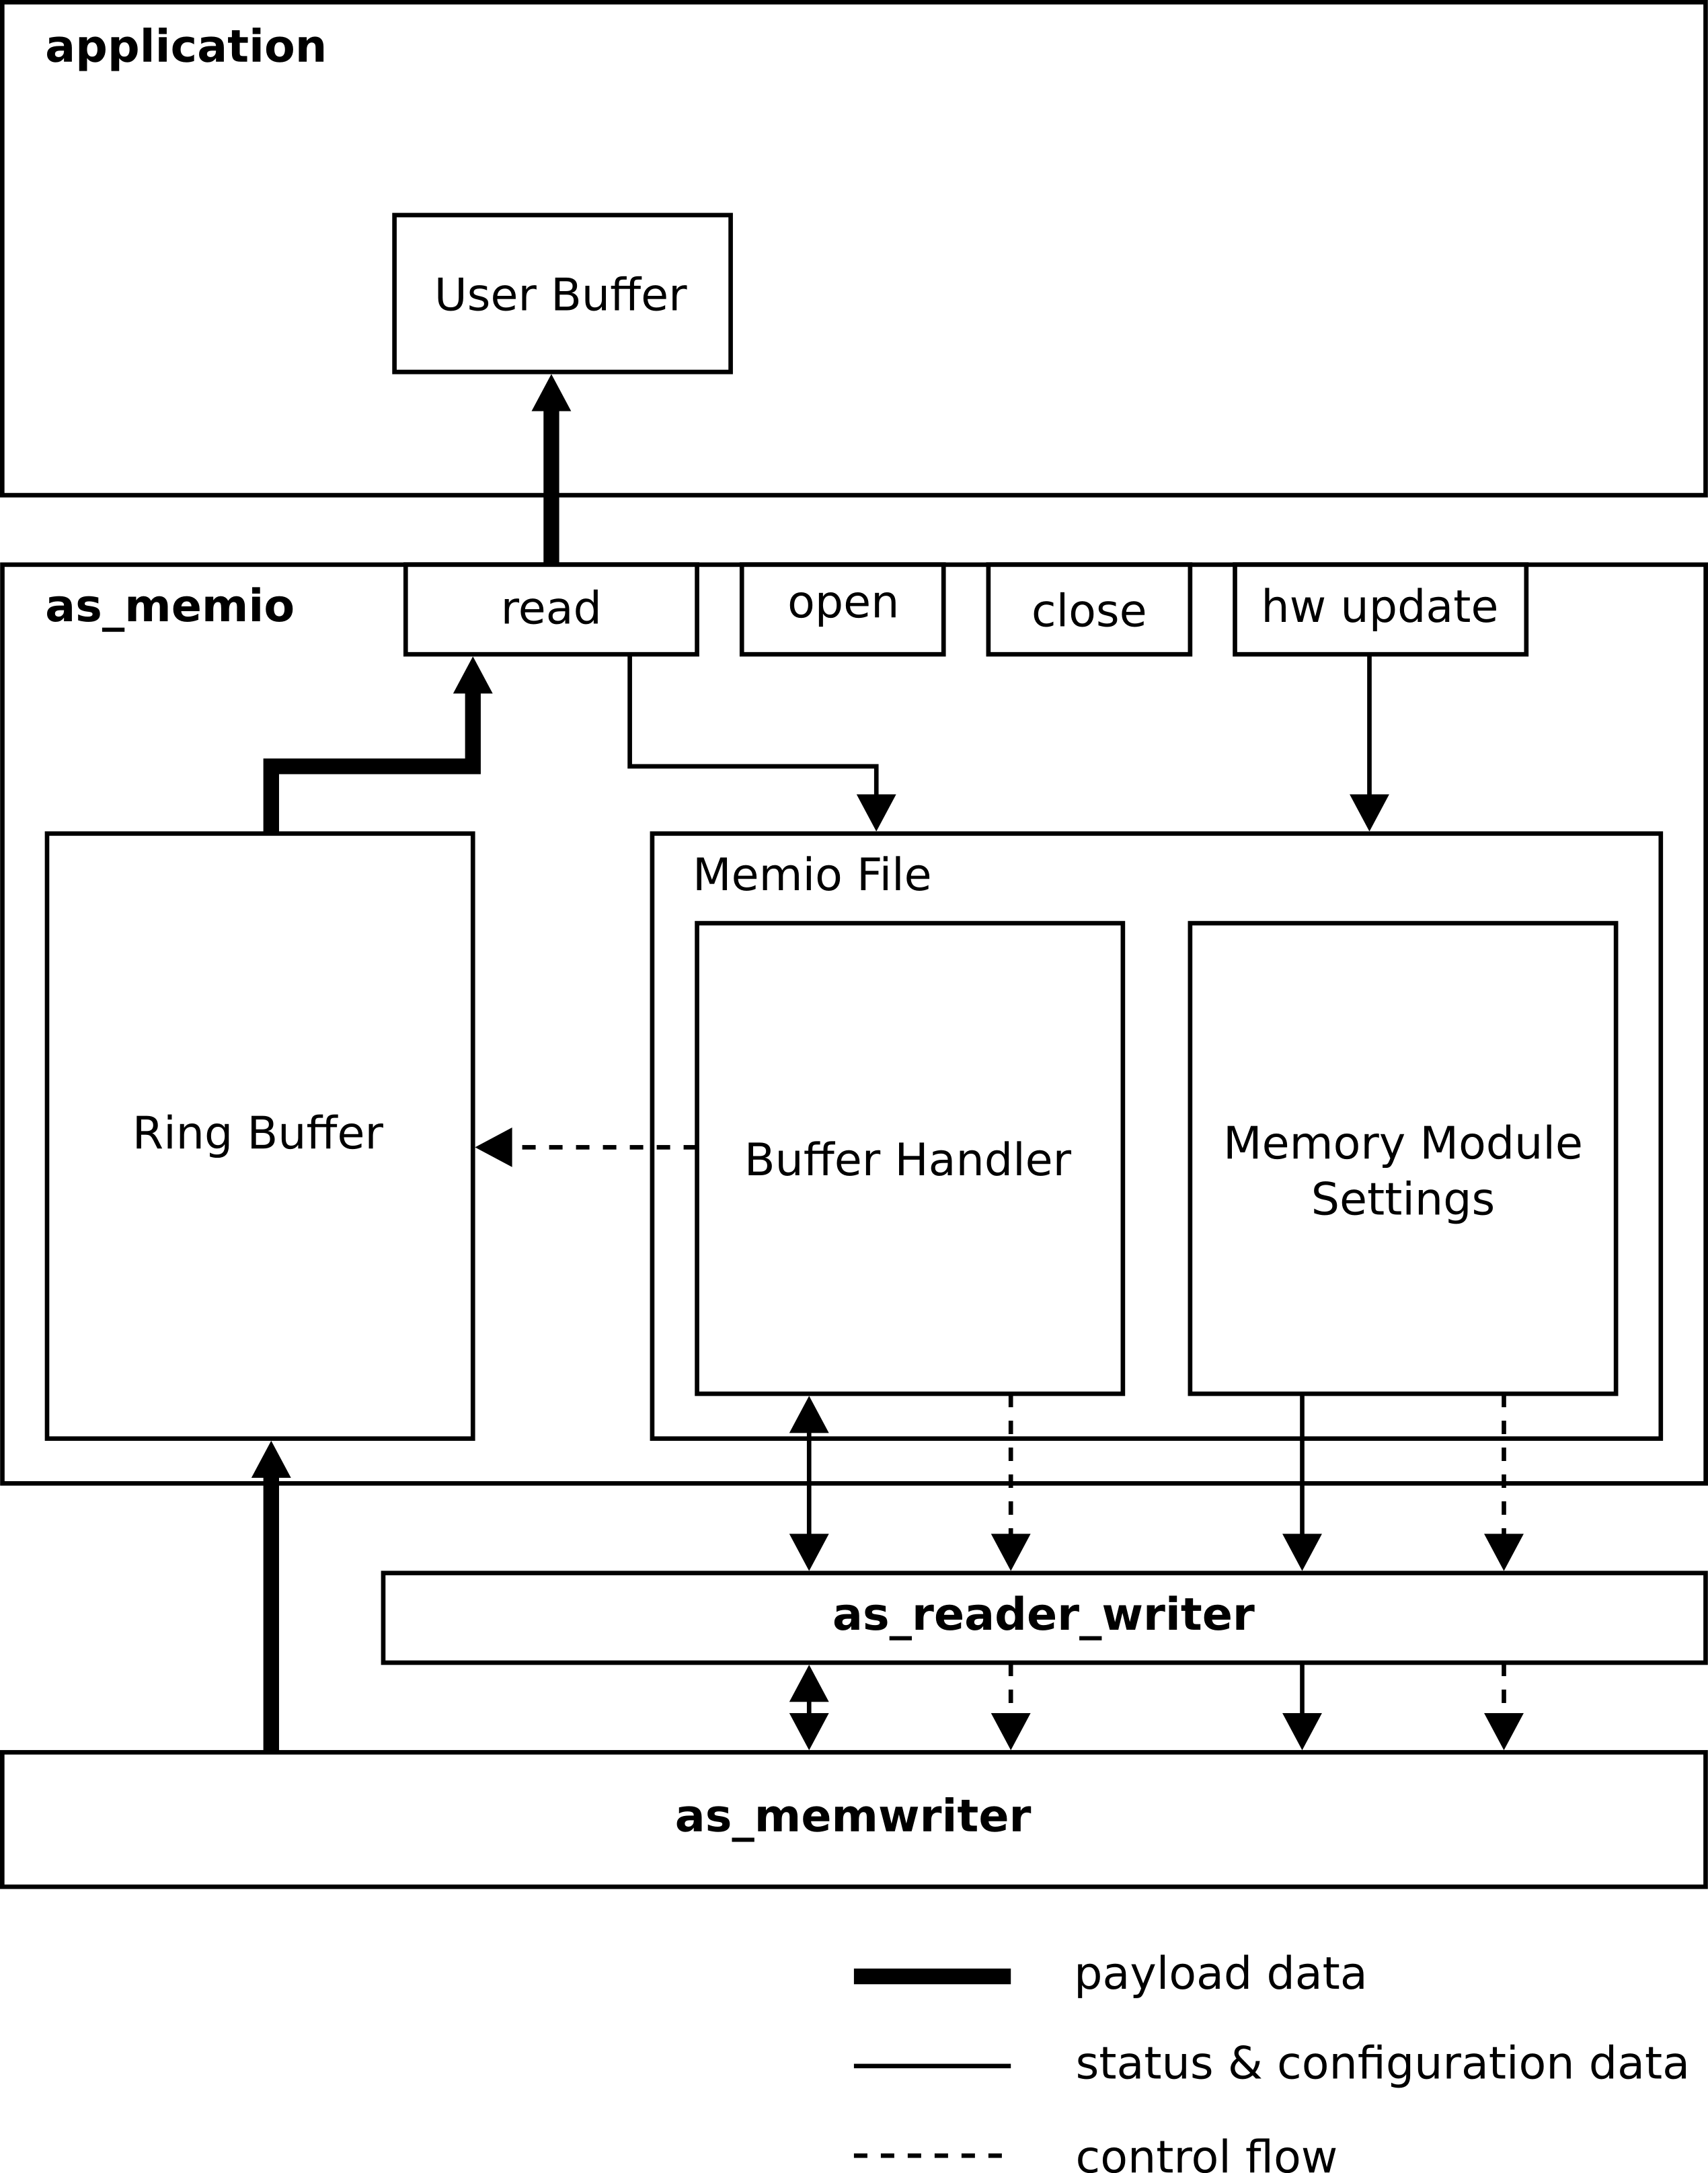
\includegraphics[width=0.6\linewidth,clip]{figs/memio.png}
    \caption{Architecture of the \texttt{as\_memio} module and its software/hardware interaction}
    \label{fig:memio}
\end{figure}

\subsubsection{Compile-Time Options}\label{ch:07-basic-modules-as_memio-options}
% buffer size in byte
% safety distance in byte (transfer size)
\begin{longtable}[ht]{|l|l|l|}
    \hline
    \multicolumn{1}{|c|}{\textbf{Name}} & \multicolumn{1}{c|}{\textbf{Range}} & \multicolumn{1}{c|}{\textbf{Description}}\\
    \hline
    
    \parbox{5cm}{\small{AS\_MEMIO\_DEFAULT\_}\\\small{INTERFACE\_WIDTH}} & Positive integer value & \parbox{5cm}{\ \\
        Sets the default bit width for ALL (!) memory module bus interfaces (usually 32 or 64 bit).\\
        This parameter is likely to be dropped in a future version of \texttt{as\_memio}.\\
    }\\
    \hline
    
    \parbox{5cm}{\small{AS\_MEMIO\_DEFAULT\_}\\\small{MAX\_BURST\_LENGTH}} & Positive integer value & \parbox{5cm}{\ \\
        Sets the default burst length in byte for ALL (!) memory modules (usually 256).\\
        This parameter is likely to be dropped in a future version of \texttt{as\_memio}.\\
    }\\
    \hline
    
    \parbox{5cm}{\small{AS\_MEMIO\_DEFAULT\_}\\\small{HW\_TRANSFER\_SIZE}} & Positive integer value & \parbox{5cm}{\ \\
        Sets the default \textit{transfer size} in byte for ALL (!) \texttt{as\_memio} modules.\\
        The \textit{transfer size} is the minimum \textit{section size} to be configured for the \texttt{as\_memwriter}.\\
        Prevents data loss at the \textit{FIFO Buffer} which may occur due to too small \textit{sections}.\\
    }\\
    \hline
    
    \parbox{5cm}{\small{AS\_MEMIO\_DEFAULT\_}\\\small{FIFO\_BUFFER\_SIZE}} & Positive integer value & \parbox{5cm}{\ \\
        Sets the default \textit{Ring Buffer} size in byte for ALL (!) \texttt{as\_memio} modules.\\
        Increasing the size allows the memory module to transfer more data for a single configuration.\\
    }\\
    \hline
    
\end{longtable}

\subsubsection{Register Space}

The module described does not contain any memory-mapped control or status registers, since it is a software module.

\subsubsection{Behavior}\label{ch:07-basic-modules-as_memio-behavior}

% open
In order to establish a connection between a memory module and \texttt{as\_memio}, its \textit{open} function has to be called, named \texttt{as\_memio\_open}.
Here, the address of the memory module has to be provided, which is internally used for calls to the functions of the \texttt{as\_reader\_writer} driver.
By providing the direction of the data flow via the \texttt{flags} parameter, either a \texttt{as\_memreader} or \texttt{as\_memwriter} is associated with the instance of \texttt{as\_memio}.
The \texttt{as\_memio} module is not able to determine the module type based on the address of the memory module.
Alternatively, a pointer to a configuration structure of the type \texttt{as\_memio\_config\_t} can be provided to overwrite the default settings for this \texttt{as\_memio} instance (see \ref{ch:07-basic-modules-as_memio-options}).
If a NULL pointer is provided, the default settings are used instead.
Within the \texttt{as\_memio\_open} function, the \textit{Ring Buffer} and \textit{Memio File} are allocated.
Subsequently, the static settings of the associated memory module are initialized, such as the \texttt{max burst length}.
Lastly, the memory module is reset and the pointer to the \textit{Memio File} is returned to the user for referencing to this instance of \texttt{as\_memio}, similar to a file pointer of the POSIX \textit{open} function.
The contents of the \textit{Memio File} are hidden from the user.

% read
The function \texttt{as\_memio\_read} is used for transferring data from hardware to software.
Next to the \textit{Memio File} pointer, a \textit{User Buffer} and the desired number of bytes have to be provided.
The requested number of bytes are copied to this buffer and therefore has to be of appropriate size.
First, the \texttt{as\_memio\_read} function is checks the current status of the \texttt{as\_memwriter} module.
The \texttt{current hw addr} is read, which determines the current location within the \textit{Ring Buffer}, where the \texttt{as\_memwriter} writes to.
Additionally, if the \texttt{pending go} bit field of the \texttt{control} register is not set, the next \textit{section} is programmed, as long as there is enough empty space within the \textit{Ring Buffer}.
All addresses up to \texttt{current hw addr} have been served by the hardware module.
The actual amount of data available in the \textit{Ring Buffer} is determined by using this address in combination with the last address copied to a \textit{User Buffer} for a previous call to \texttt{as\_memio\_read}.
Figure~\ref{fig:memio_buffer_read} shows how the available data within the \textit{Ring Buffer} is determined. 
The \texttt{current hw addr} is shown as \textit{hw} and the following address after the last copy process to the \textit{User Buffer} as \textit{sw}.
Both are represented within the \textit{Buffer Handler} of \texttt{as\_memio}.
If the number of bytes in the \textit{Ring Buffer} is not equal to the requested one, the smaller number of bytes is copied.
The address of \textit{sw} is increased for each copied byte to the \textit{User Buffer} throughout the lifetime of the \texttt{as\_memio} instance.
If either \textit{hw} or \textit{sw} exceeds the upper boundary of the \textit{Ring Buffer}, it is set to its start address again (bottom).
The \textit{Buffer Handler} prevents buffer over- and underflow due to one pointer overtaking the other.
After completing \texttt{as\_memio\_read}, the actual number of copied bytes is returned to the caller and the \textit{User Buffer} contains the data.

\begin{figure}[ht]
    \centering
    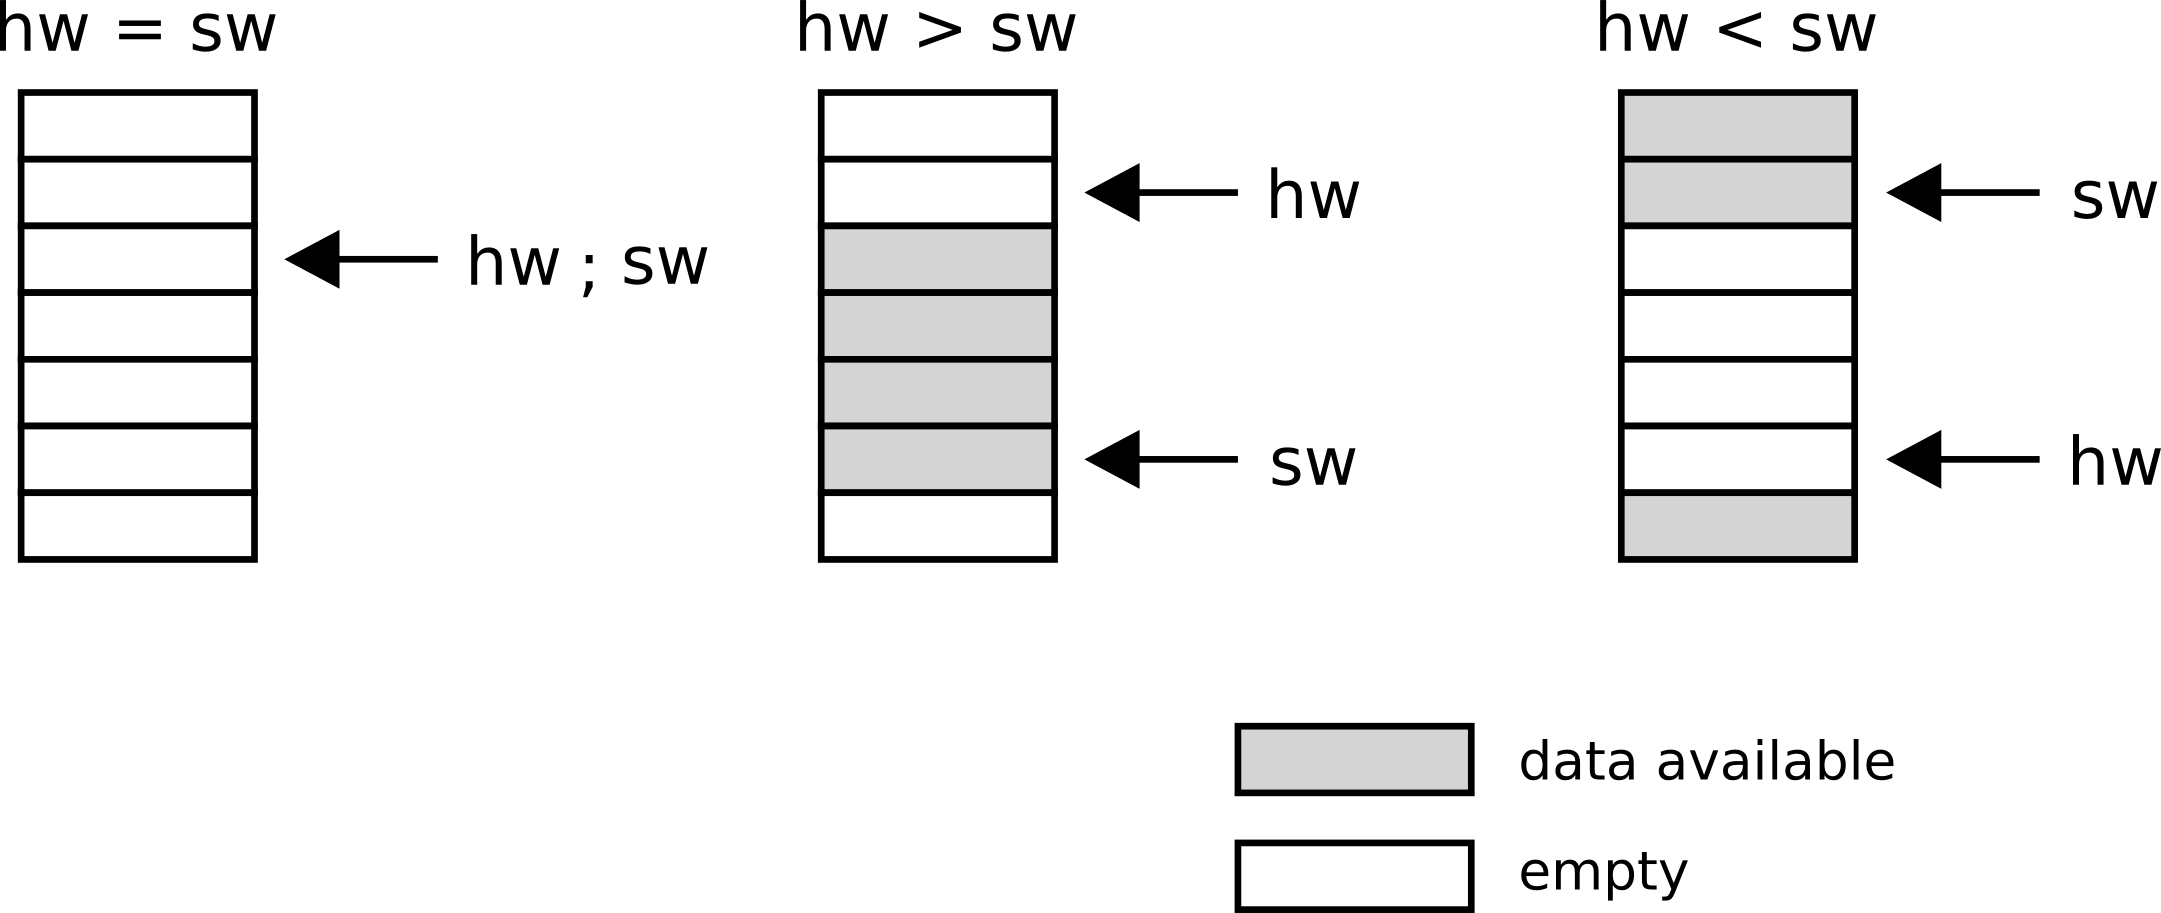
\includegraphics[width=0.6\linewidth,clip]{figs/memio_buffer_read.png}
    \caption{Determining the available amount of data within the \textit{Ring Buffer} for \texttt{as\_memio\_read}}
    \label{fig:memio_buffer_read}
\end{figure}

% write
The \texttt{as\_memio\_write} function operates in a similar way but data is copied from the \textit{User Buffer} to the empty slots of the \textit{Ring Buffer}.
Figure~\ref{fig:memio_buffer_write} shows how the available addresses within the \textit{Ring Buffer} are determined.
Since a \texttt{as\_memreader} is associated with this function it can only be configured once data is available in the \textit{Ring Buffer}.
Therefore, \texttt{current hw addr} is read after copying the data from the \textit{User Buffer} as well as programming the next \textit{section} in case the \texttt{pending go} field of the \texttt{control} register is not set.
Although \texttt{as\_memio} has been able to copy all data to the \textit{Ring Buffer}, the actual data transfer may not yet be completed after \texttt{as\_memio\_write} returns.

\begin{figure}[ht]
    \centering
    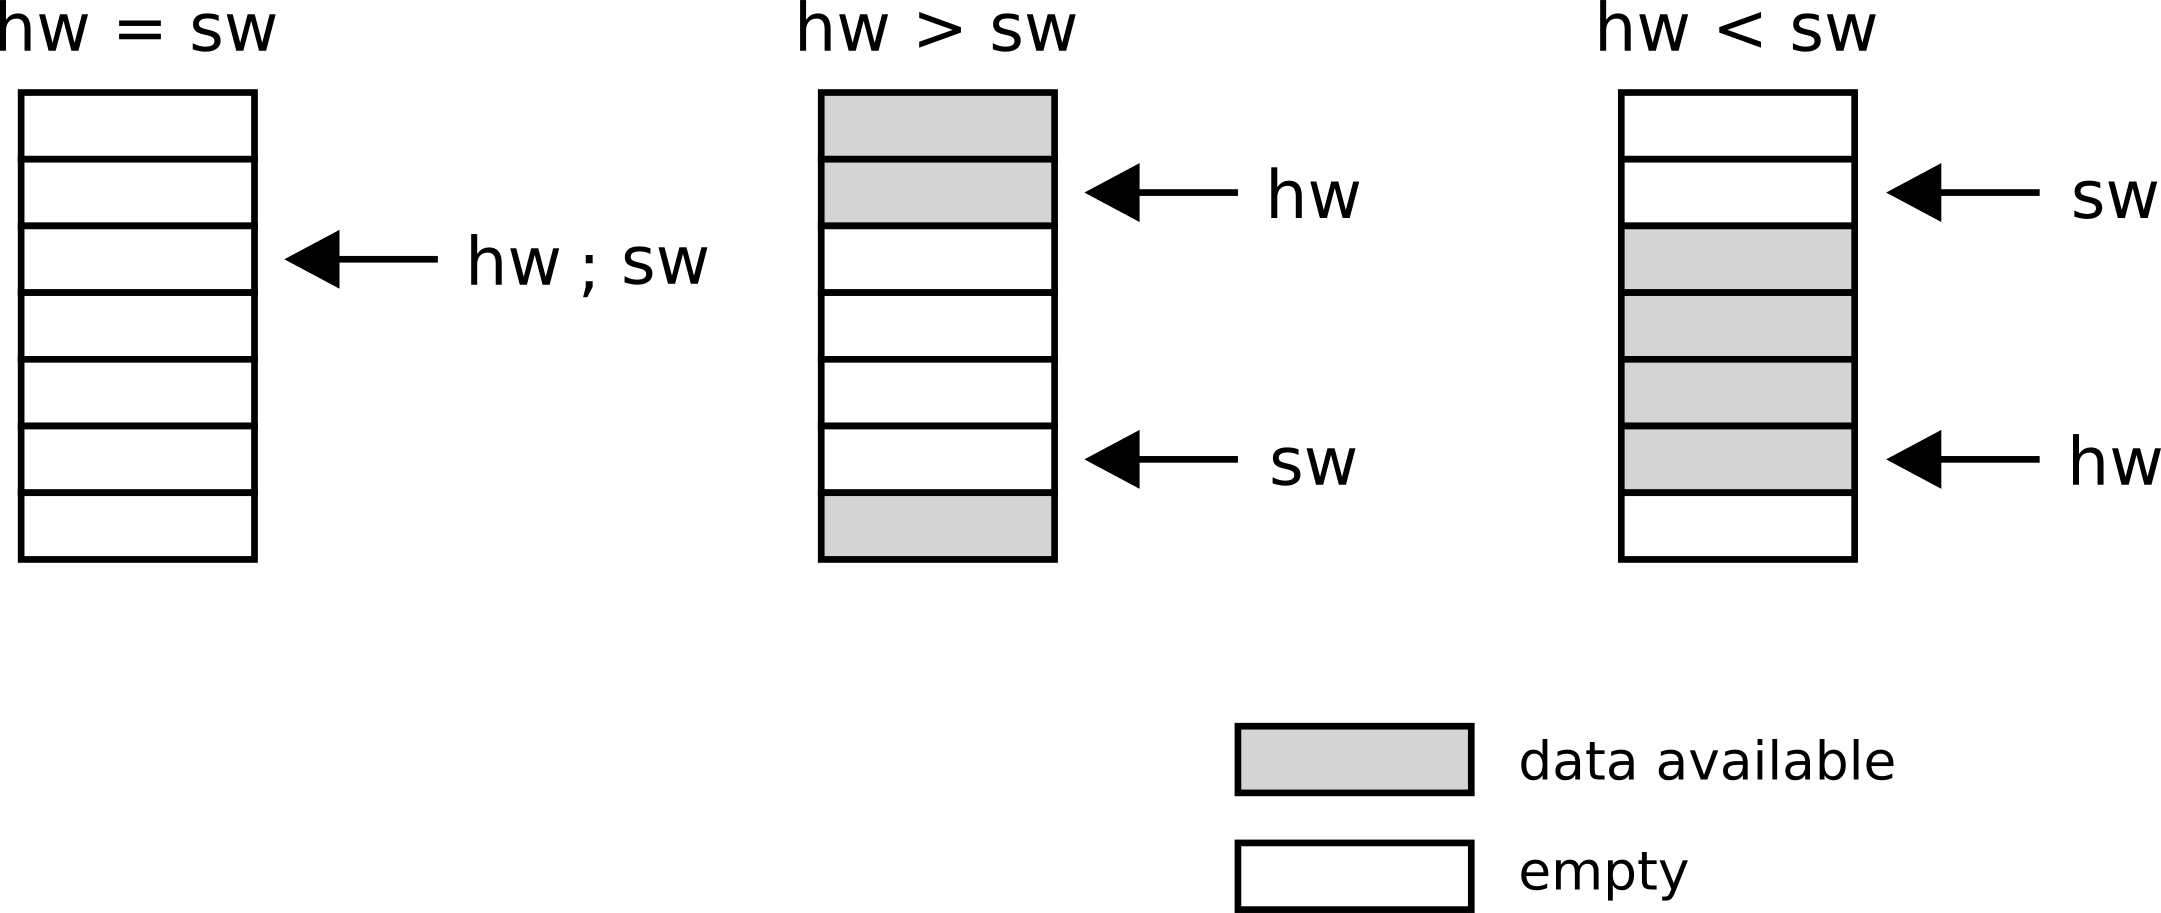
\includegraphics[width=0.6\linewidth,clip]{figs/memio_buffer_write.png}
    \caption{Determining the available amount of data within the \textit{Ring Buffer} for \texttt{as\_memio\_write}}
    \label{fig:memio_buffer_write}
\end{figure}

% hw update
The \texttt{as\_memio} module implicitly programs its associated memory module when calling either \texttt{as\_memio\_read} or \texttt{as\_memio\_write}.
Although sufficient in most cases, explicitly programming the memory module is required if the last data transfer between the \textit{Ring Buffer} and \textit{User Buffer} results in a boundary crossing by the hardware module.
Since the memory modules only support a single \textit{section} which has to consist of physically concurrent addresses, wrapping around the \textit{Ring Buffer} requires programming the memory modules twice.
This is shown in Figure~\ref{fig:memio_buffer_read} and~\ref{fig:memio_buffer_write} for "hw $>$ sw", where the first \textit{section} has to be programmed starting from \textit{hw} up to the end of the \textit{Ring Buffer} and the second on from the beginning.
The second \textit{section} can be programmed by using the \texttt{as\_memio\_hw\_update} function.
When the instance of \texttt{as\_memio} is associated with a \texttt{as\_memreader}, it prevents data from getting "stuck" in the \textit{Ring Buffer} which could cause the image processing chain to wait indefinitely for data to arrive.
For the \texttt{as\_memwriter}, it prevents a potential overflow of its \textit{FIFO Buffer} due to not being able to transfer the data to the \textit{Ring Buffer}.

% Transfer size
Although the \texttt{as\_memwriter} is able to request the preceding hardware module to suspend data transfers when its \textit{FIFO Buffer} is full, not all modules are able to suspend their transfers (e.g. camera).
For this reason, the \texttt{as\_memio} module uses a \textit{transfer size} when programming the \textit{section} size for the \texttt{as\_memwriter} to cater for continuous data streams.
The \textit{transfer size} is the minimum number of bytes which have to be transferred by the \texttt{as\_memwriter} to prevent overflows of its \textit{FIFO Buffer} due to setting up a too small \textit{section}.
This is mainly relevant when the \texttt{as\_memwriter} is about to cross the upper boundary of the \textit{Ring Buffer} of the \texttt{as\_memio} module.
Since two \textit{sections} have to be programmed when wrapping around the \textit{Ring Buffer}, the first one has to be big enough to give the software time to program the second one.
The \textit{FIFO Buffer} of the \texttt{as\_memwriter} must not overflow during this given time window.
The \textit{Ring Buffer} of \texttt{as\_memio} has to be a multiple of the \textit{transfer size}.

% close
The call to \texttt{as\_memio\_close} deletes a no longer required instance of the \texttt{as\_memio} module.
Here, the associated memory module is reset and all acquired resources are returned. 
Since the \textit{Memio File} no longer exists after this point, it can no longer be used. 

All calls to the functions of the \texttt{as\_memio} module are nonblocking and therefore return immediately even if the request could not be fulfilled.
This may require to call \texttt{as\_memio\_read} or \texttt{as\_memio\_write} more than once to transfer the desired number of bytes.



\subsubsection{Application Notes}
Figure~\ref{lst:memio_simple} shows the setup of the \texttt{as\_memio} module using default settings.

\begin{footnotesize}
    \lstset{style=CStyle, caption={Using \texttt{as\_memio} for transferring data from hardware to software}}
    \begin{lstlisting}[label=lst:memio_simple]
    
    #define IMAGE_RES           640*480
    int n;
    
    void *user_buffer = as_malloc(IMAGE_RES);
    
    /******* Setting up as_memio *******/
    
    struct as_memio_file_s *memio_read_fp = \
        as_memio_open(AS_ADDR(AS_MODULE_BASEREG_MEMWRITER_0), \
            NULL, O_WRONLY);
    
    
    /************** Data transfer **************/
    
    n = 0;
    
    while(n < IMAGE_RES) {
    n += as_memio_read(memio_read_fp, user_buffer+n, IMAGE_RES-n)
    }
    
    \end{lstlisting}
\end{footnotesize}
